\newpage
\appendix
\onecolumn

In this part, we introduce the appendix. We introduce the additional experiments in Sec.\ref{ap:exp} including backgrounds, setups, hyperparameters selections, and some figures of experiments. We introduce the theoretical proofs in Sec.\ref{ap:proof}.

% \paragraph{Limitations.} To avoid the dual drifts, we propose the virtual dual updates to align the old dual variables with the new global model. This requires those dual variables of non-active clients to be updated on the global server, yielding more storage costs. As a trade-off, our method applies additional variable assistance to greatly improve the stability of such algorithms. It also is an interesting future study to approximate the virtual dual update on the local clients.

\section{Additional Experiments}
\label{ap:exp}
\subsection{Benchmarks}
\label{ap:fedpdsam}
We select 6 classical state-of-the-art~(SOTA) benchmarks as baselines in our paper, including (a) \textit{primal}: \textit{FedAvg}~\cite{mcmahan2017communication}, \textit{SCAFFOLD}~\cite{karimireddy2020scaffold}, \textit{FedCM}~\cite{xu2021fedcm}, \textit{FedSAM}~\cite{qu2022generalized}; (b) \textit{primal dual}: \textit{FedADMM}~\cite{wang2022fedadmm}, \textit{FedDyn}~\cite{wang2022fedadmm}, \textit{FedSpeed}~\cite{sun2023fedspeed}. We mainly focus on infrastructure improvements instead of combinations of techniques. In the \textit{primal} group, \textit{SCAFFOLD} and \textit{FedCM} alleviate ``client drift'' via variance reduction and client-level momentum correction respectively. \textit{FedSAM} introduce the \textit{Sharpeness Aware Minimization}~(SAM)~\cite{foret2020sharpness} in vanilla \textit{FedAvg} to smoothen the loss landscape. In the \textit{primal dual} group, we select the \textit{FedDyn} as the stable basis under partial participation. We also show the instability of the vanilla \textit{FedADMM} to show the negative impacts of the ``\textit{dual drift}''. \textit{FedSpeed} introduces the \textit{SAM} in vanilla \textit{FedADMM}\ /\ \textit{FedDyn}. We also test the variant of \textit{SAM} version of our proposed \textit{A-FedPD} method, which is named \textit{A-FedPDSAM}.

\begin{algorithm}[H]
\small
	\renewcommand{\algorithmicrequire}{\textbf{Input:}}
	\renewcommand{\algorithmicensure}{\textbf{Output:}}
	\caption{A-FedPDSAM Algorithm}
    \begin{multicols}{2}
	\begin{algorithmic}[1]
		\REQUIRE $\theta^0$, $\theta_i^0$, $T$, $K$, $\lambda_i^0$, $\rho$
		\ENSURE global average model\\
            \STATE \textbf{Initialization} : $\theta_i^0=\theta^0$, $\lambda_i^0=0$.
            \FOR{$t = 0, 1, 2, \cdots, T-1$}
            \STATE randomly select active clients set $\mathcal{P}^t$ from $\mathcal{C}$
            \FOR{client $i \in \mathcal{P}^t$ \textbf{in parallel}}
            \STATE receive $\lambda_i^t, \theta^t$ from the global server
            %\STATE (A2) {\color{red}{$\lambda_i^{t+1} = \lambda_i^t + \rho(w_i^{t+1} - w^t)$}}
            \STATE $\theta_i^{t+1} = \textit{LocalTrain}(\lambda_i^t, \theta^t, \eta^t, K)$
            %\STATE $\lambda_i^{t+1} = \lambda_i^t + \rho(w_i^{t+1} - w^t)$
            \STATE send $\theta_i^{t+1}$ to the global server 
            \ENDFOR
            %\STATE $\lambda^{t+1} = \lambda^t + \frac{1}{C}\sum_{i\in \mathcal{N}^t}\rho(w_{i}^{t+1}-w^t)$
            \STATE $\overline{\theta}^{t+1} = \frac{1}{P}\sum_{i\in\mathcal{P}^t}\theta_i^{t+1}$
            \STATE $\lambda_i^{t+1}=\textit{D-Update}(\lambda_i^t, \theta^t, \theta_i^{t+1}, \overline{\theta}^{t+1}, \mathcal{P}^t)$
            \STATE $\overline{\lambda}^{t+1} = \frac{1}{C}\sum_{i\in\mathcal{C}}\lambda_i^{t+1}$
            \STATE $\theta^{t+1} = \overline{\theta}^{t+1} + \frac{1}{\rho} \overline{\lambda}^{t+1}$
            \ENDFOR
            \STATE return global average model
	\end{algorithmic}
    \textit{$\diamondsuit$ LocalTrain}: (Optimize Eq.(\ref{lagrangian}))
    \begin{algorithmic}[1]
	\REQUIRE $\lambda_i^t$, $\theta^t$, $\eta^t$, $K$
	\ENSURE $\theta_{i,K}^t$
        \FOR{$k = 0, 1, 2, \cdots, K-1$}
        \STATE select a minibatch $\mathcal{B}$
        \STATE $g_{i,k}^t=\nabla f_i(\theta_{i,k,t} + \rho\frac{\nabla f_i(\theta_{i,k,t}, \mathcal{B})}{\Vert\nabla f_i(\theta_{i,k,t}, \mathcal{B})\Vert}, \mathcal{B})$
        \STATE $\theta_{i,k+1}^t = \theta_{i,k}^t - \eta^t(g_{i,k}^t + \lambda_i^t + \rho(\theta_{i,k}^t - \theta^t))$
        \ENDFOR
	\end{algorithmic}

    \textit{$\diamondsuit$ D-Update}:~(update dual variables)
    \begin{algorithmic}[1]
    \REQUIRE $\lambda_i^t, \theta^t, \theta_i^{t+1}, \overline{\theta}^{t+1}, \mathcal{P}^t$
	\ENSURE $\lambda_i^{t+1}$
    \IF{$i\in\mathcal{P}^t$}
    \STATE $\lambda_i^{t+1} = \lambda_i^{t} + \rho_t(\theta_i^{t+1} - \theta^t)$
    \ELSE 
    \STATE $\lambda_i^{t+1} = \lambda_i^{t} + \rho_t(\overline{\theta}^{t+1} - \theta^t)$
    \ENDIF
    \end{algorithmic}
\end{multicols}
\vspace{-0.3cm}
\end{algorithm}

\subsection{Hyperparameters Selection}
We first introduce the hyperparameter selections. To fairly compare the efficiency of the benchmarks, we fix the most of hyperparameters, including the initial global learning rate, the initial learning rate, the weight decay coefficient, and the local batchsize. The other hyperparameters are selected properly on a grid search within the valid range. The specific hyperparameters of specific methods are defined in the experiments. We report the corresponding selections of their best performance, which is summarized in the following Table~\ref{tb:hyper}.

\begin{table}[h]
\centering
\vspace{-0.2cm}
\caption{Hyperparameters selections of benchmarks.}
\small
%\renewcommand\arraystretch{1.5}
\scalebox{0.8}{
\begin{tabular}{|c|c|c|c|c|c|c|c|}
\toprule
 & Grid Search & FedAvg & FedCM & SCAFFOLD & FedSAM & FedDyn & FedSpeed \\
\midrule
global learning rate & [0.1, 1.0] & \multicolumn{6}{c|}{1.0} \\
local learning rate & [0.01, 0.1, 1.0] & \multicolumn{6}{c|}{0.1} \\
weight decay & [0.0001, 0.001, 0.01] & \multicolumn{6}{c|}{0.001} \\
\midrule
learning rate decay & [0.995, 0.998, 0.9998, 1] & 0.998 & 0.998 & 0.998 & 0.998 & 0.998\ /\ 1 & 0.998\ /\ 1 \\
batchsize & [10, 20, 50, 100] & 50 & 50 & 50 & 50 & 20\ /\ 50 & 50 \\
\midrule
client-level momentum & [0.05, 0.1, 0.2, 0.5] & & 0.1 & & & & \\
proxy coefficient & [0.001, 0.01, 0.1, 1.0] & & & & & 0.1\ /\ 0.001  & 0.1 \\
SAM perturbation & [0.01, 0.05, 0.1, 0.5] & & & & 0.05 & & 0.1 \\
SAM eps & [1e-2, 1e-5, 1e-8] & & & & 1e-2 & & all \\
\bottomrule
\end{tabular}}
\label{tb:hyper}
%\vspace{-0.3cm}
\end{table}

The global learning rate is fixed in our experiments. Though \citet{asad2020fedopt} propose to adopt the double learning rate decay both on the global server and local client can make training more efficient, we find some methods will easily over-fit under a global learning rate decay. For the weight decay coefficient, we recommend to adopt $0.001$. Actually, we find that adjusting it still can improve the performance of some specific methods. One of the most important hyperparameters is learning rate decay. Generally, we use $d^T = 1\ /\ 0.8\ /\ 0.1\ /\ 0.005$ to select the proper $d$ as a decayed coefficient, which means the level of the initial learning rate will be decayed after $T$ communication rounds. We follow previous studies to fix the learning rate within the communication round. Another important hyperparameter is the batchsize. In our experiments, we fixed the local interval which means the fixed local iterations. Due to the sample size being fixed, different batchsizes mean different training epochs. Generally speaking, training epochs always decide the optimization level on the local optimum. A too-long interval always leads to overfitting to the local dataset and falling into the serious ``client drift'' problem~\citep{karimireddy2020scaffold}. In our experiments, we control it to stop when the local client is optimized well enough, i.e., a proper loss or accuracy. For the specific hyperparameters for each method, we directly grid search from the selections. For \textit{A-FedPDSAM} method, the selections are consistent with the \textit{FedDyn} and \textit{FedSpeed} methods except for the learning rate decay is fixed as 0.998. To alleviate the ``dual drift'', we properly reduce the proxy coefficient for the \textit{FedDyn} on those difficult tasks to maintain stable training.


\subsection{Dataset and Splitting}
\begin{figure*}[t]
\vskip -0.05in
\centering
    \subfigure[IID splitting.]{
        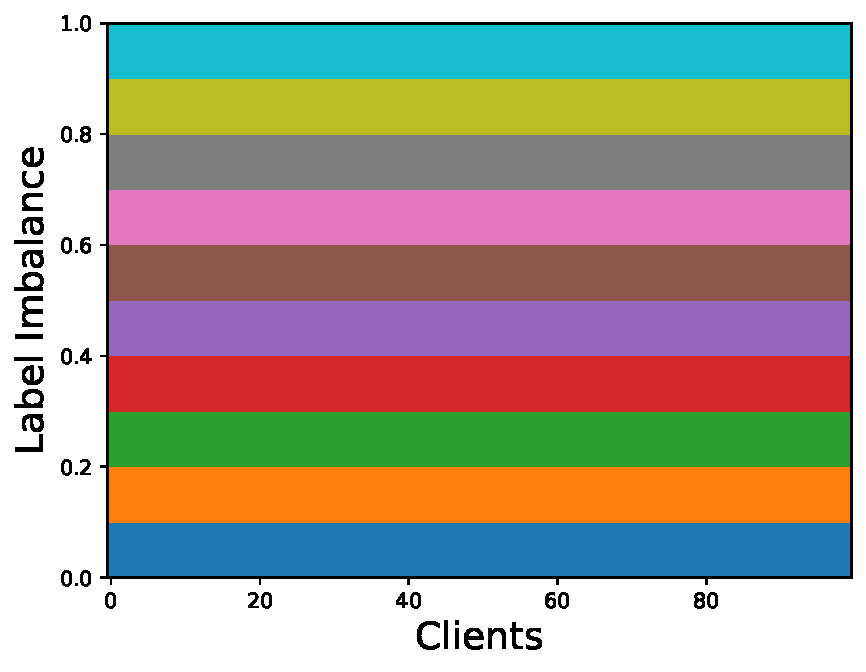
\includegraphics[width=0.33\textwidth]{figure/distribution_iid.pdf}}\!\!\!\!
    \subfigure[Dir-1.0 splitting.]{
	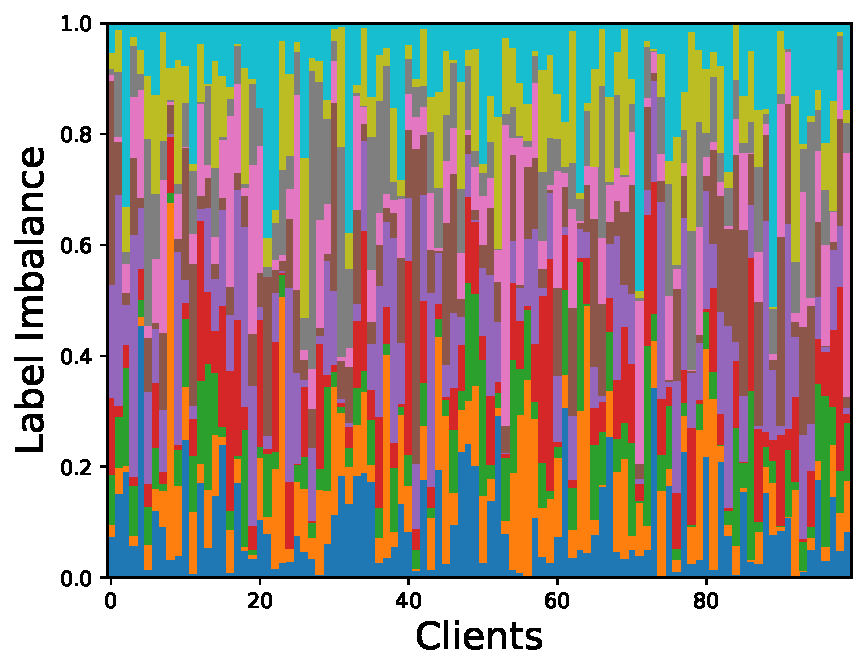
\includegraphics[width=0.33\textwidth]{figure/distribution_1.0.pdf}}\!\!\!\!
    \subfigure[Dir-0.1 splitting.]{
	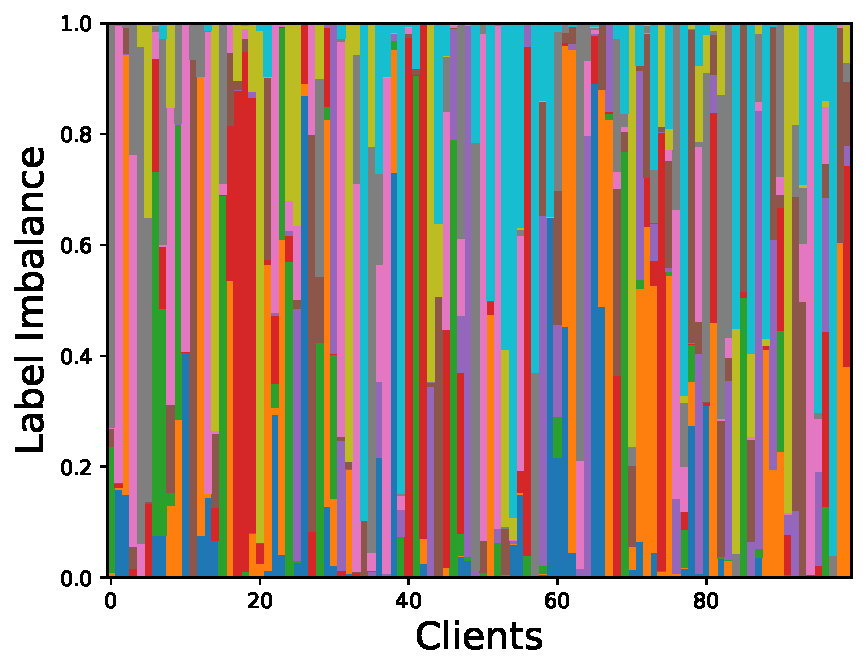
\includegraphics[width=0.33\textwidth]{figure/distribution_0.1.pdf}}
\vskip -0.1in
\caption{Label ratios under different splitting manners. Different color means the samples are in different labels. We show the different splitting distributions on a total of 100 clients.}
\label{label imbalance}
\vskip -0.1in
\end{figure*}
We use the CIFAR-10\ /\ 100 datasets to validate the efficiency, which is widely used to verify the federated efficiency~\citep{mcmahan2017communication,karimireddy2020scaffold,li2020federated,xu2021fedcm,durmus2021federated,gong2022fedadmm,wang2022fedadmm,fan2022fedskip,caldarola2022improving,sun2023fedspeed,sun2023dynamic,li2023dfedadmm,fan2024locally,fan2024federated}. The total dataset of both contain 50,000 training samples and 10,000 test samples of 10\ /\ 100 classes. Each is a colorful image in the size of 32$\times$32. We follow the training as the vanilla SGD to add data augmentation without additional operations.

\textbf{Label Heterogeneity.} For the dataset splitting, we adopt the label imbalanced splitting under the Dirichlet manners. We first generate a distribution matrix and then generate a random number to sample each data. To further enhance the local heterogeneity, we also adopt the sampling with replacement, which means one data sample may exist on several clients simultaneously. This is more related to real-world scenarios because of the local unknown dataset distribution. We generate the matrices in Fig.~\ref{label imbalance} to show their distribution differences. We can clearly see that Dir-0.1 introduces a very large heterogeneity in that there is almost one dominant class in a client. Dir-1.0 handles approximately 3 classes in one client. Actually, in practical scenarios, label imbalance may be the most popular heterogeneity because we often expect both the local task and local dataset to be still unknown to others. For instance, client $i$ may be an expert on task $A$, and client $j$ may be an expert on another task $B$. To combine the tasks $A$ and $B$, if we can directly merge them with a training policy without beforehand knowing the tasks, then it must further enhance local privacy.

\textbf{Brightness Heterogeneity.} To further simulate the real-world manners, we allow different clients to change the brightness and ratios of different color channels. This corresponds to different sources of data collected by different local clients. We show some samples in Fig.~\ref{brightness imbalance} to show how different they are on different clients. Specifically, after splitting the local dataset, we will calculate the average brightness of each local dataset. Then we generate a noise from Gaussian to randomly change the brightness and one of the color channels, which means that even similar samples have large color differences on different clients.
\begin{figure}[h]
\vskip -0.1in
\centering
    \subfigure{
        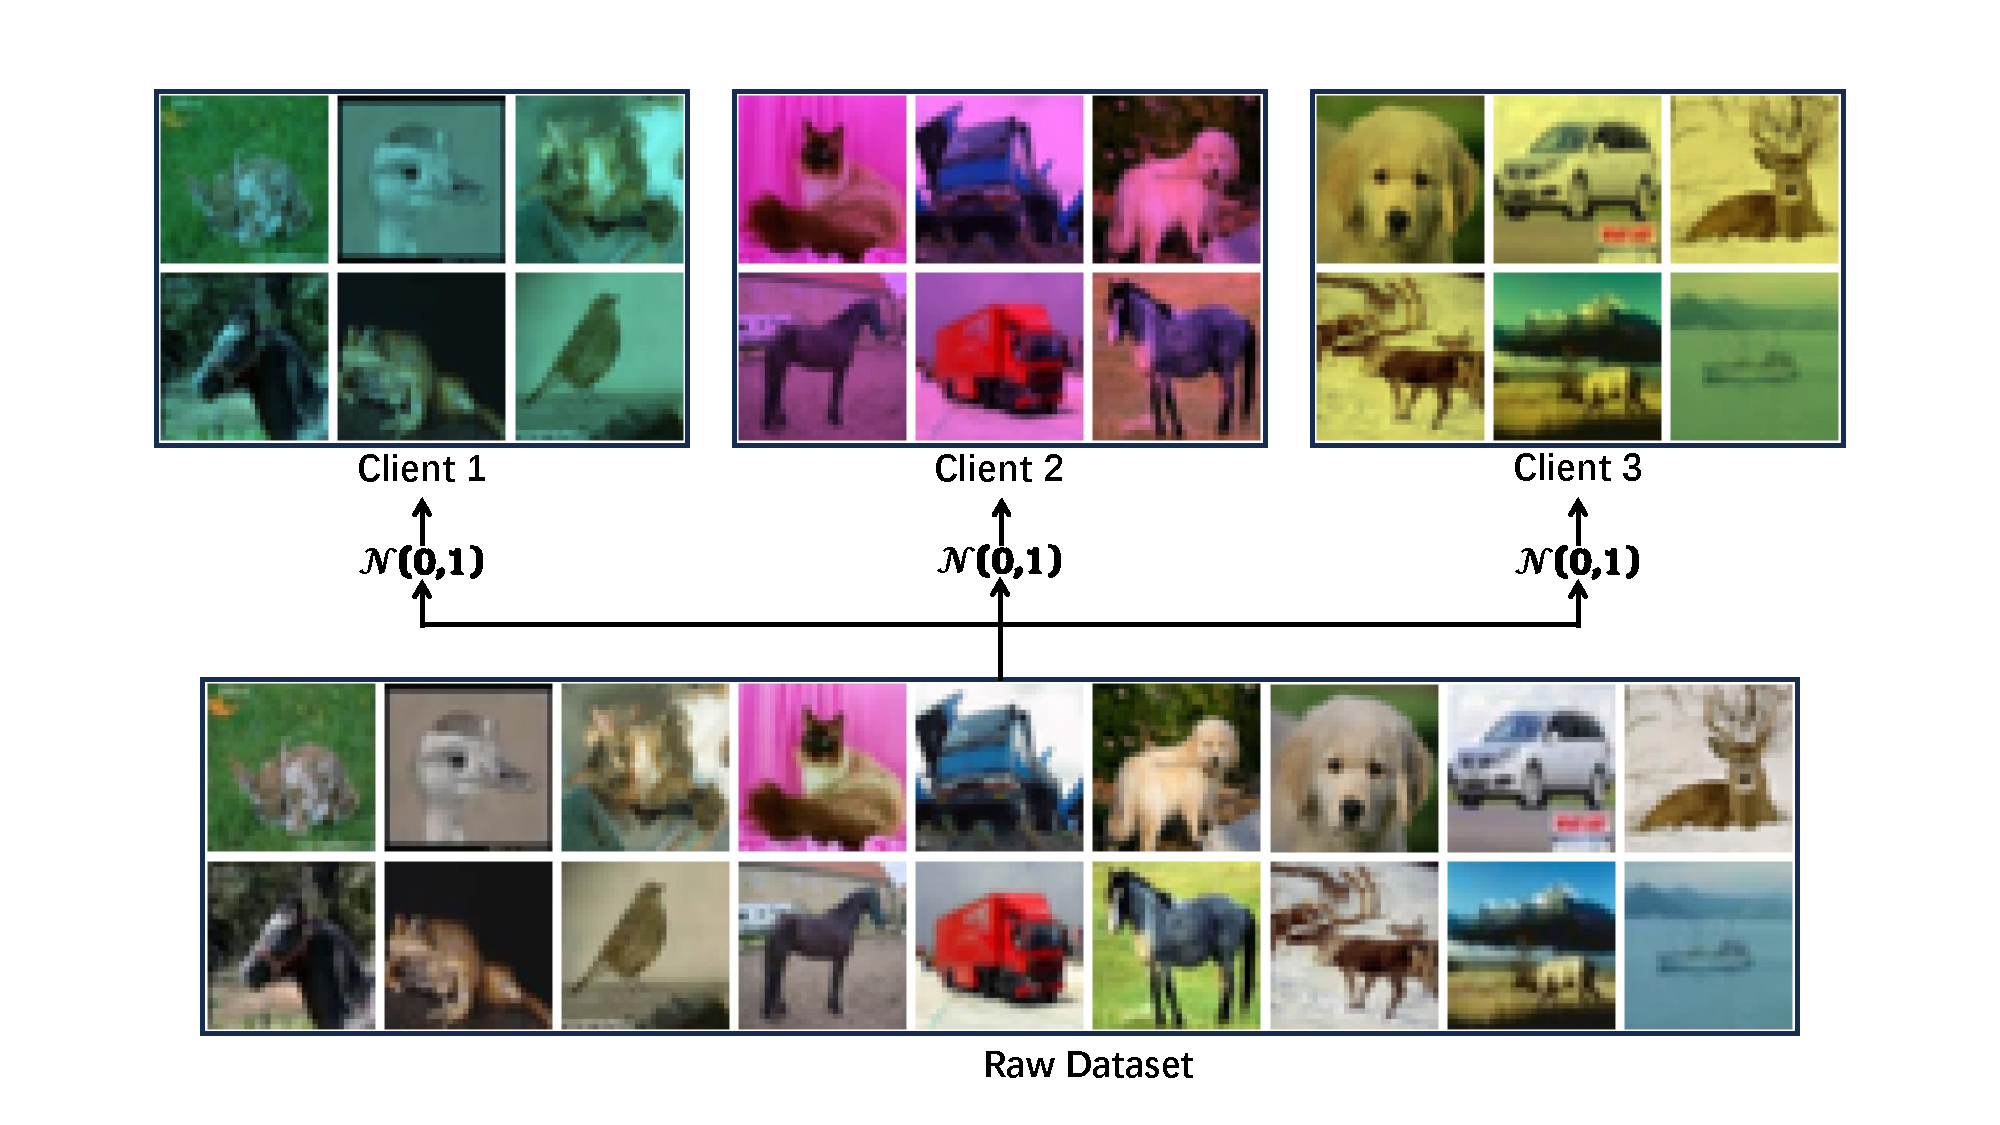
\includegraphics[width=0.9\textwidth]{figure/class.pdf}}
\vskip -0.1in
\caption{Introducing the brightness biases to different clients. We calculate the average brightness to control each sample to a proper state. Each client will randomly sample a Gaussian noise to perturb the local samples.}
\label{brightness imbalance}
\vskip -0.1in
\end{figure}

\subsection{Additional Experiments}
\subsubsection{Some Training Curves}
\begin{figure}[h]
\vskip -0.05in
\centering
    \subfigure[Loss IID.]{
        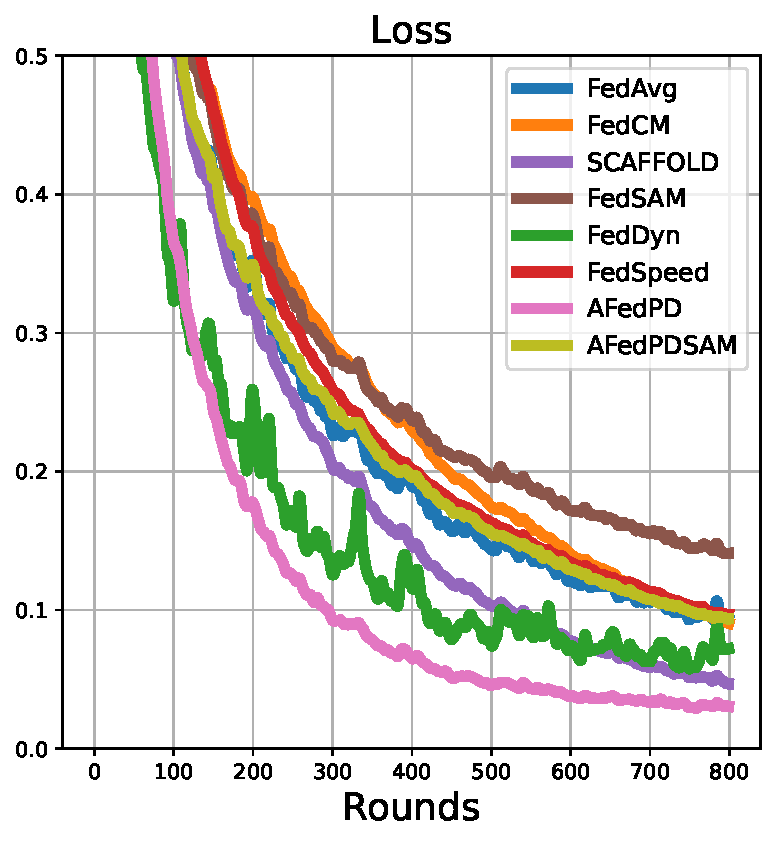
\includegraphics[width=0.23\textwidth]{figure/loss_lenet_CIFAR10_IID_.pdf}}
    \subfigure[Loss Dir-1.0.]{
	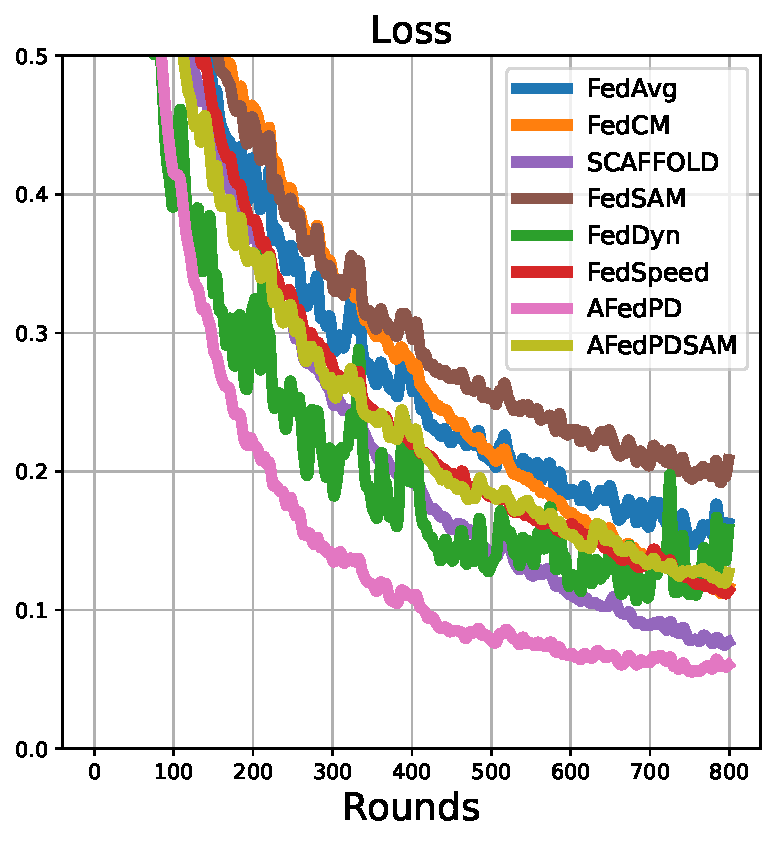
\includegraphics[width=0.23\textwidth]{figure/loss_lenet_CIFAR10_Dirichlet_1.0.pdf}}
    \subfigure[Loss Dir-0.6.]{
        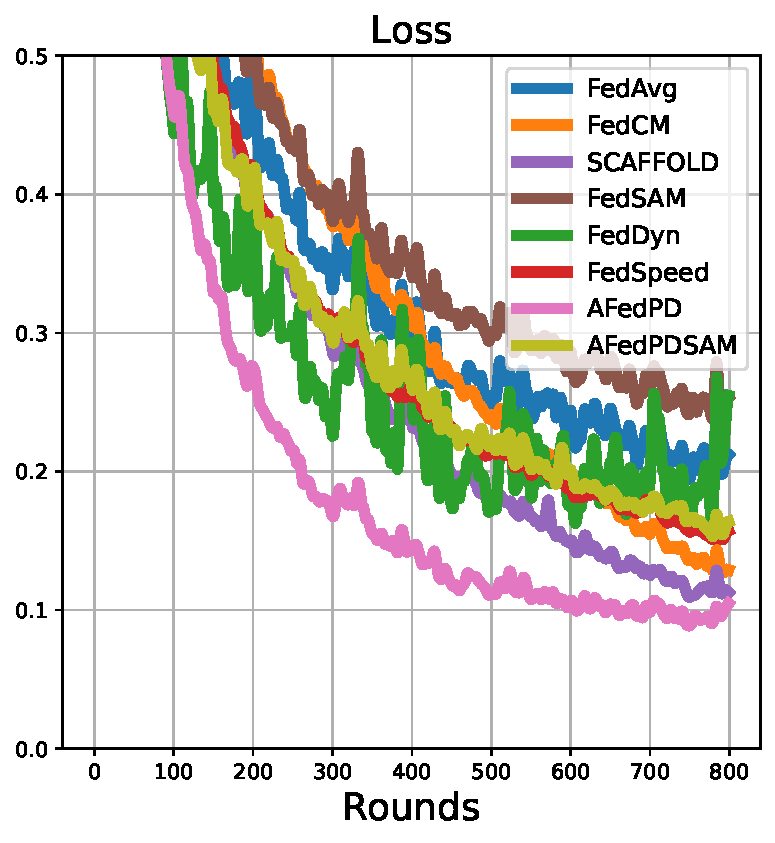
\includegraphics[width=0.23\textwidth]{figure/loss_lenet_CIFAR10_Dirichlet_0.6.pdf}}
    \subfigure[Loss Dir-0.1.]{
	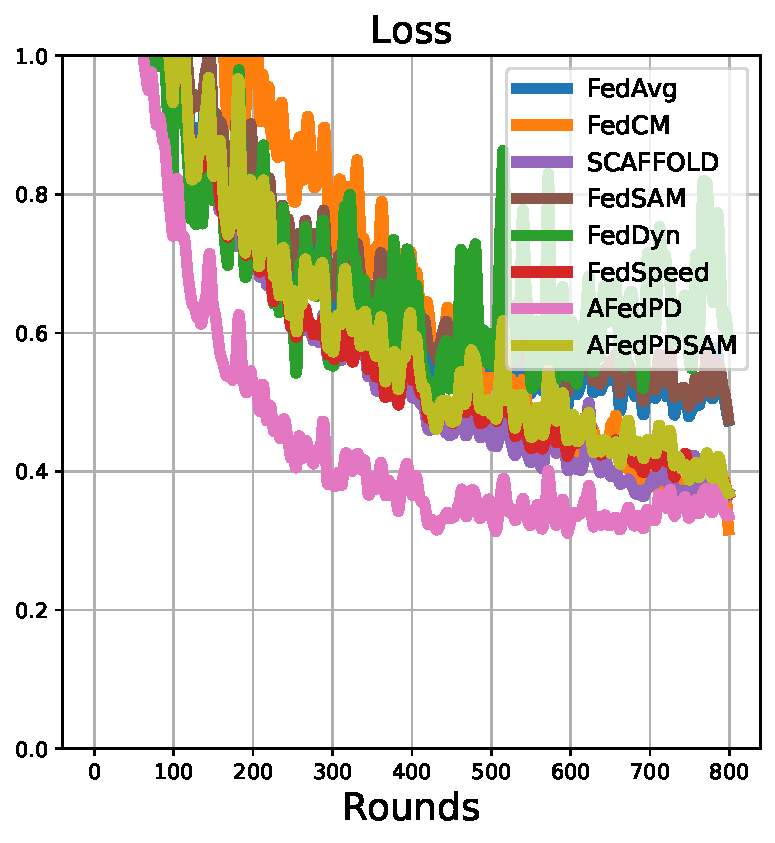
\includegraphics[width=0.23\textwidth]{figure/loss_lenet_CIFAR10_Dirichlet_0.1.pdf}}
    \subfigure[Acc IID.]{
        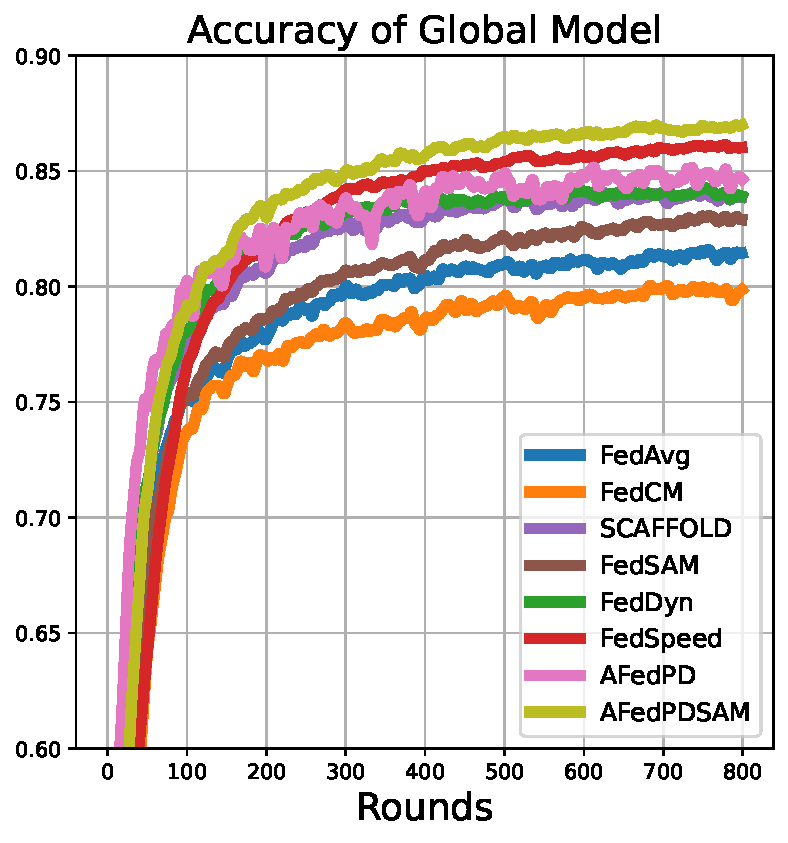
\includegraphics[width=0.23\textwidth]{figure/acc_lenet_CIFAR10_IID_.pdf}}
    \subfigure[Acc Dir-1.0.]{
	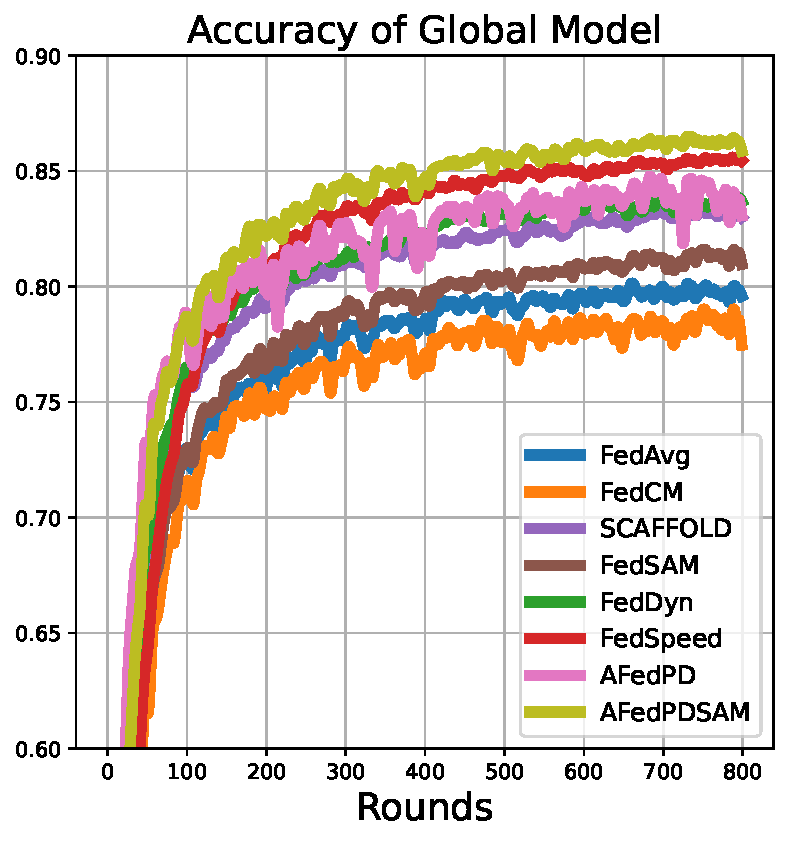
\includegraphics[width=0.23\textwidth]{figure/acc_lenet_CIFAR10_Dirichlet_1.0.pdf}}
    \subfigure[Acc Dir-0.6.]{
        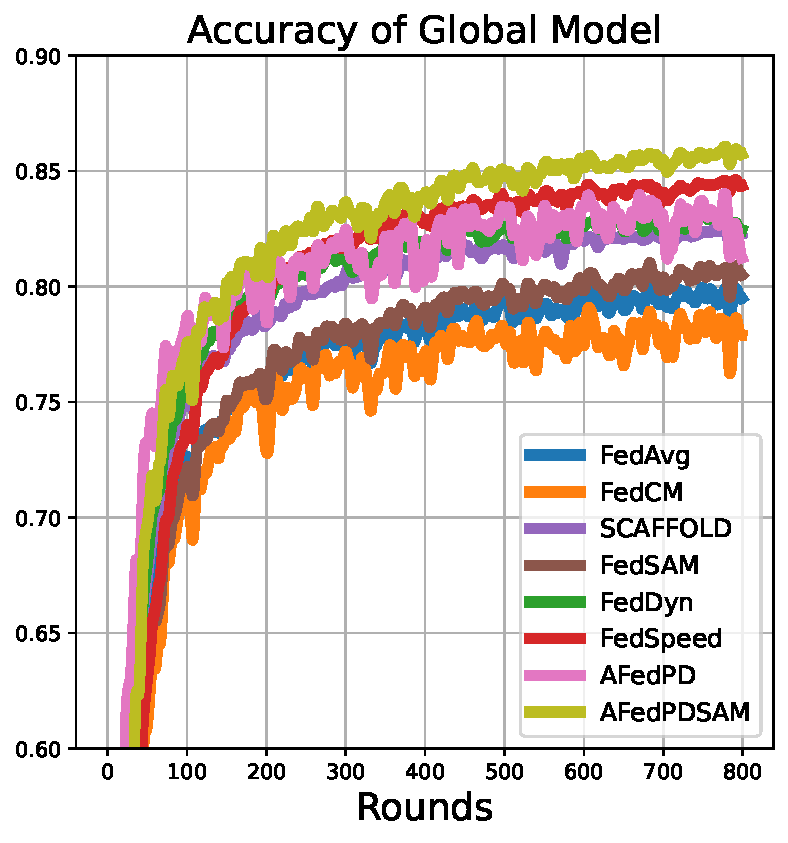
\includegraphics[width=0.23\textwidth]{figure/acc_lenet_CIFAR10_Dirichlet_0.6.pdf}}
    \subfigure[Acc Dir-0.1.]{
	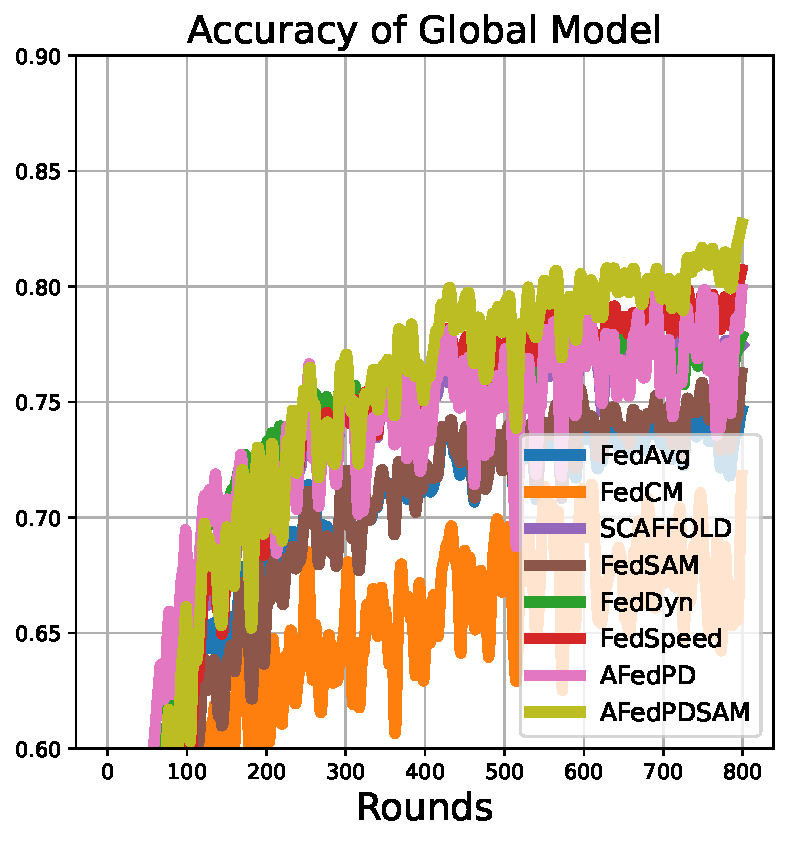
\includegraphics[width=0.23\textwidth]{figure/acc_lenet_CIFAR10_Dirichlet_0.1.pdf}}
\vskip -0.1in
\caption{Loss and accuracy curves in the experiments.}
\label{curves}
\vskip -0.1in
\end{figure}
In Figure~\ref{curves} we can see some experiment curves. From the (a), (b), (c), and (d), we can clearly see that the \textit{A-FedPD} method achieves the fastest convergence rate on each setup. Due to the virtual update on the dual variables, we can treat those unparticipated clients as virtually trained ones. This empowers the \textit{A-FedPD} method with a great convergence speed. Especially on the IID dataset, due to the local datasets being similar~(drawn from a global distribution), the expectation of the updated averaged models is the same as that of the updated local model with lower variance. Then we could approximate the local dual update as the global one. This greatly speeds up the training time. We also can see the fast rate of the \textit{FedDyn} method. However, due to its lagging dual update, it will be slower than the \textit{A-FedPD} method. As for the \textit{SAM} variant, it introduces an additional perturbation step that could avoid overfitting. Therefore, its loss does not drop quickly because of the additional ascent step.

From the (e), (f), (g), and (h), we can clearly see the improvements of \textit{A-FedPD} and \textit{A-FedPDSAM} methods. From the basic version, \textit{A-FedPD} could achieve higher performance due to the virtual dual updates. After incorporating \textit{SAM}, local clients could efficiently alleviate overfitting. The global model becomes more stable and could achieve the SOTA results. We will learn the consistency performance in the next part.

\newpage
\subsubsection{Primal Residual and Dual Residual}
In the \textit{primal dual} methods, due to the joint solution on both the primal and dual problems, it leads to an issue that both residuals should maintain a proper ratio. Therefore, the quantity of global updates in the training could be considered as a residual for the dual feasibility condition. The same, the constraint itself could be considered as the primal residual. Then we consider Eq.(\ref{consensus_objective}) objectives. The constraint is the global consensus level $\theta - \theta_i$ and the global update is $\theta^{t+1} - \theta^t$. To generally express them, we define the primal residual $p_r^t = \frac{1}{C}\sum_{i}\Vert \theta^t - \theta_i^t\Vert$ and the dual residual $d_r^t = \rho\Vert \theta^{t} - \theta^{t-1}\Vert$. Actually, the primal residual could be considered as the consistency, and the dual residual could be considered as the update. In the training, if we focus more on the dual residual, it leads to a fast convergence on an extremely biased objective that is far away from the true optimal. If we focus more on the primal residual, the local training cannot perform normally for its strong regularizations. Therefore, we must maintain stable trends on both $p_r$ and $d_r$ to implement stable training. In this part, we study the relationships between primal and dual residuals.
\begin{figure}[h]
\vskip -0.05in
\centering
    \subfigure[Residuals on the CIFAR-10 test.]{
        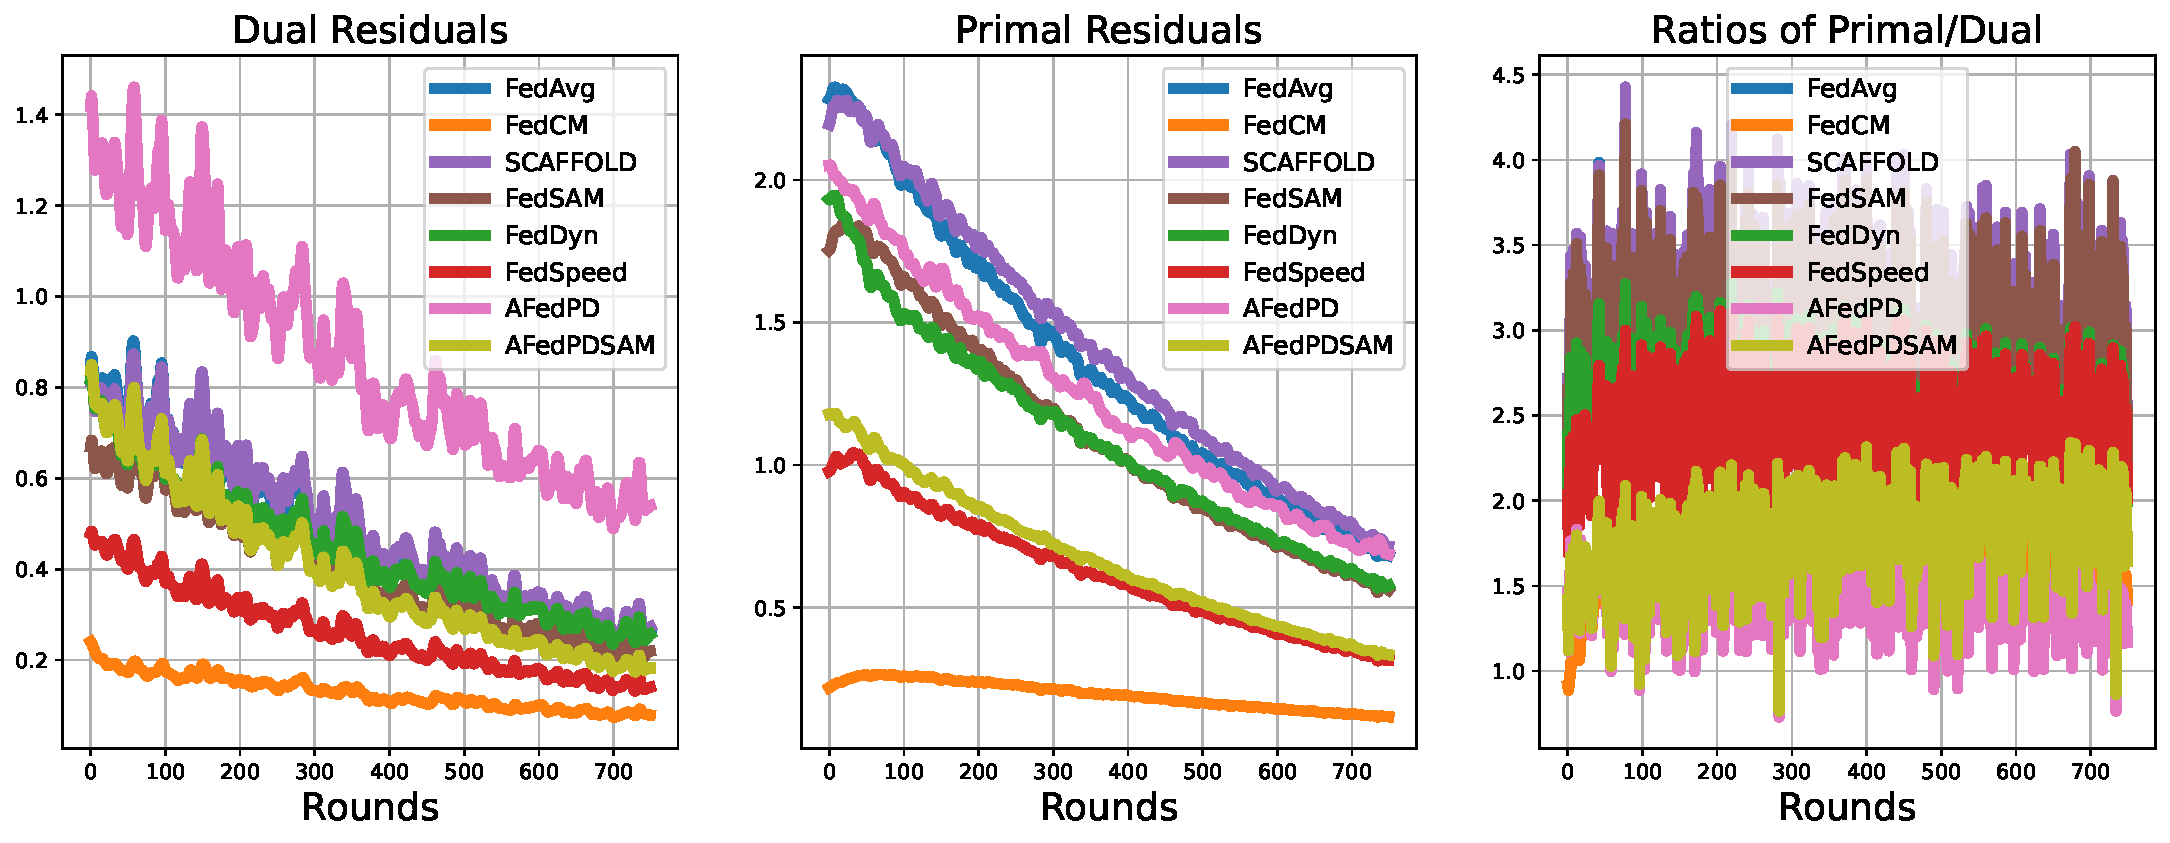
\includegraphics[width=0.9\textwidth]{figure/cifar10_residuals.pdf}}
    \subfigure[Residuals on the CIFAR-100 test.]{
        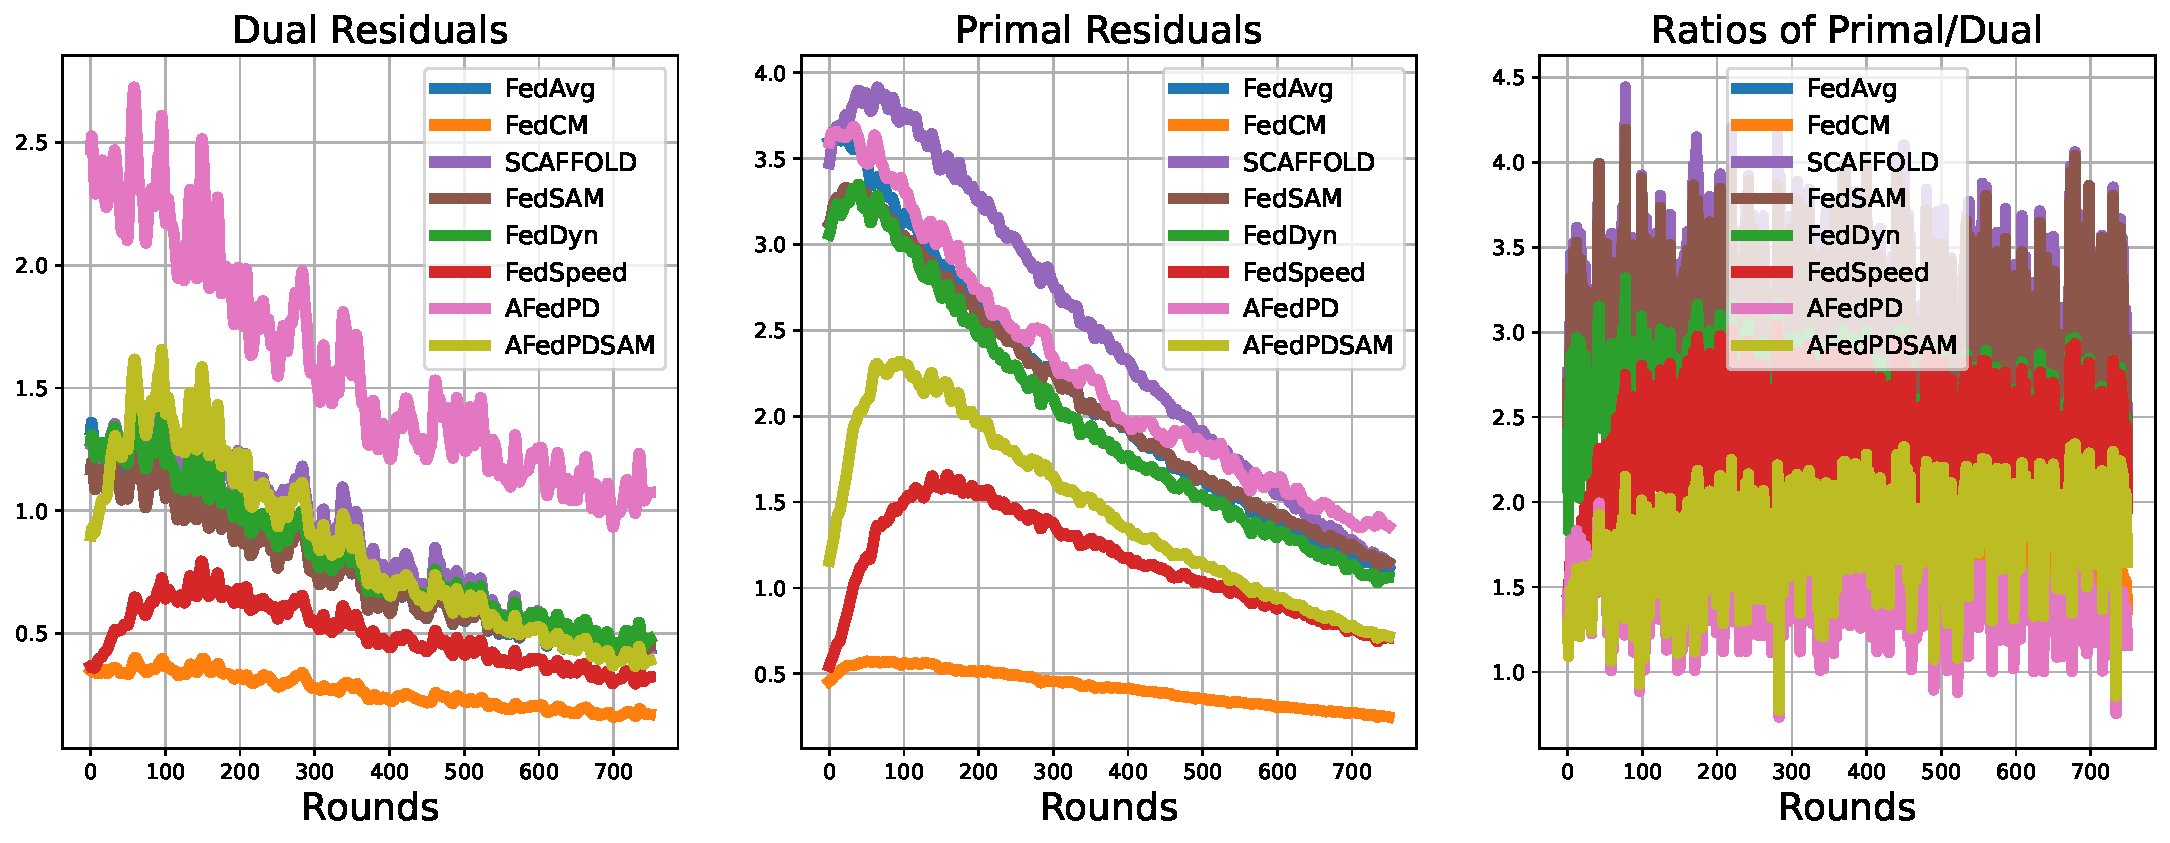
\includegraphics[width=0.9\textwidth]{figure/cifar100_residuals.pdf}}
\vskip -0.1in
\caption{Loss and accuracy curves in the experiments.}
\label{residuals}
\vskip -0.1in
\end{figure}

As shown in Figure~\ref{residuals}, we can clearly see the lower stable ratio between the primal and dual residuals on the \textit{A-FedPD} and \textit{A-FedPDSAM} methods, which indicates that both the primal training and dual training are performed well simultaneously. However, the \textit{federated primal average}-based methods, i.e., \textit{FedAvg} and \textit{SCAFFOLD}, focus more on the primal training which leads to the dual residuals are too small~(dual residuals measure the global update; primal residuals measure the global consistency).


\newpage
\subsubsection{Communication Efficiency}
In this part, we learn the general communication efficiency. We fix all local intervals, clients, participation ratios, and hyperparameters for fairness. We select the different targets as the objective to calculate the communication efficiency.

\begin{table}[h]
\centering
\vspace{-0.2cm}
\caption{Communication rounds required to achieve the target accuracy.}
\vspace{0.05cm}
\small
\renewcommand\arraystretch{1.5}
\begin{tabular}{|c|ccccccc|}
\toprule
CIFAR-10 & FedAvg & SCAFFOLD & FedSAM & FedDyn & FedSpeed & A-FedPD & A-FedPDSAM \\
\midrule
81\% & 501 & 207 & 345 & 156 & 170 & 131 & 156 \\
\cmidrule(lr){2-8}
     & 1$\times$ & 2.42$\times$ & 1.45$\times$ & 3.21$\times$ & 2.94$\times$ & 3.82$\times$ & 3.21$\times$ \\
\midrule
83.5\% & - & 468 & - & 355 & 268 & 252 & 218 \\
\cmidrule(lr){2-8}
       & - & 1$\times$ & - & 1.31$\times$ & 1.74$\times$ & 1.85$\times$ & 2.14$\times$ \\
 \midrule
 CIFAR-100 & FedAvg & SCAFFOLD & FedSAM & FedDyn & FedSpeed & A-FedPD & A-FedPDSAM \\
\midrule
40\% & 772 & 162 & 572 & 173 & 222 & 123 &  126\\
\cmidrule(lr){2-8}
     & 1$\times$ & 4.76$\times$ & 1.34$\times$ & 4.46$\times$ & 3.47$\times$ & 6.27$\times$ & 6.12$\times$ \\
\midrule
49\% & - & 677 & - & 495 & 421 & 303 & 220 \\
\cmidrule(lr){2-8}
     & - & 1$\times$ & - & 1.36$\times$ & 1.61$\times$ & 2.23$\times$ & 3.07$\times$ \\
\bottomrule
\end{tabular}
\label{tb:communication efficiency}
%\vspace{-0.3cm}
\end{table}

Table~\ref{tb:communication efficiency} shows the communication efficiency among different methods on the CIFAR-10\ /\ 100 dataset trained with LeNet. We calculate the first communication round index of achieving the target accuracy for comparison. We can clearly see that the communication rounds required for training are saved a lot on the proposed \textit{A-FedPD} and \textit{A-FedPDSAM} methods. It generally accelerates the training process by at least 3$\times$ on CIFAR-10 and 6$\times$ on CIFAR-100 than the vanilla \textit{FedAvg} method. Compared with the other benchmarks, our proposed method performs stably and efficiently.

\subsubsection{Wall clock Time for Training Costs}
\label{wall=clock}
Then we further study the wall clock time required in the training. We provide the experimental setups as follows.

Platform: Pytorch 2.0.1 \quad \quad
Cuda: 11.7 \quad \quad
Hardware: NVIDIA GeForce RTX 2080 Ti
\begin{table}[h]
\centering
\vspace{-0.2cm}
\caption{Wall clock time required to train 1 round~(100 iterations) on \textbf{ResNet}.}
\vspace{0.05cm}
\small
\renewcommand\arraystretch{1.5}
\begin{tabular}{|c|ccccccc|}
\toprule
 & FedAvg & SCAFFOLD & FedSAM & FedDyn & FedSpeed & A-FedPD & A-FedPDSAM \\
\midrule
s\ /\ round & 22.06 & 36.01 & 39.21 & 34.03 & 56.10 & 37.61 & 60.63 \\
\cmidrule(lr){2-8}
            & 1$\times$ & 1.63$\times$ & 1.77$\times$ & 1.54$\times$ & 2.54$\times$ & 1.70$\times$ & 2.74$\times$ \\
\bottomrule
\end{tabular}
\label{tb:wall-clock time on resnet}
%\vspace{-0.3cm}
\end{table}

\begin{table}[h]
\centering
\vspace{-0.4cm}
\caption{Wall clock time required to train 1 round~(100 iterations) on \textbf{LeNet}.}
\vspace{0.05cm}
\small
\renewcommand\arraystretch{1.5}
\begin{tabular}{|c|ccccccc|}
\toprule
 & FedAvg & SCAFFOLD & FedSAM & FedDyn & FedSpeed & A-FedPD & A-FedPDSAM \\
\midrule
s\ /\ round & 9.82 & 11.42 & 12.53 & 11.76 & 13.61 & 11.71 & 13.90 \\
\cmidrule(lr){2-8}
            & 1$\times$ & 1.16$\times$ & 1.27$\times$ & 1.19$\times$ & 1.38$\times$ & 1.19$\times$ & 1.41$\times$ \\
\bottomrule
\end{tabular}
\label{tb:wall-clock time on lenet}
%\vspace{-0.3cm}
\end{table}

Actually, the LeNet is too small for the GPU and the training time does not achieve the capacity, which leads to the close time costs in Table~\ref{tb:wall-clock time on lenet}. We recommend referring to the cost ratio on the ResNet~(Table~\ref{tb:wall-clock time on resnet}), which is much closer to the real algorithmic efficiency.























\newpage
\section{Proofs.}
\label{ap:proof}

In this part, we mainly show the proof details of the main theorems in this paper. We will reiterate the background details in Sec.\ref{ap:preliminaries}. Then we introduce the important lemmas used in the proof in Sec.\ref{ap:important lemmas}, and show the proof details of the main theorems in  Sec.\ref{ap:proofs of theorem}.

\subsection{Preliminaries}
\label{ap:preliminaries}

Here we reiterate the background details in the proofs. To understand the stability efficiency, we follow \citet{hardt2016train,lei2020fine,zhou2021towards,sun2023understanding} to adopt the uniform stability analysis in our analysis. Through refining the local subproblem of the solution of the Augmented Lagrangian objective, we provide the error term of the primal and dual terms and their corresponding complexity bound in FL.

Before introducing the important lemmas, we re-summarize the pipelines in the analysis. According to the federated setups, we assume a global server coordinates a set of local clients $\mathcal{C}\triangleq\left\{i\right\}_{i=1}^C$ to train one model. Each client has a private dataset $\mathcal{S}_i=\left\{\zeta_{ij}\right\}_{j=1}^S$. We assume that the global joint dataset is the union of $\{\mathcal{S}_1\cup\mathcal{S}_2\cup\cdots\cup\mathcal{S}_C\}$. To study its stability, we assume there is another global joint dataset that contains at most one different data sample from $\mathcal{C}$. Let the index of the different pair be $(i^\star,j^\star)$. We train two global models $\theta^T$ and $\hat{\theta}^T$ on these two global joint datasets respectively and gauge their gaps during the training process.

Then we rethink the local solution of the local augmented Lagrangian function. According to the basic algorithm, we have:
\begin{equation}
    \mathcal{L}_i(\theta, \lambda_i^t, \theta^t) = f_i(\theta) + \langle\lambda_i^t, \theta - \theta^t\rangle + \frac{\rho}{2}\Vert \theta - \theta^t\Vert^2.
\end{equation}
To upper bound its stability without loss of generality, we consider adopting the general SGD optimizer to solve the sub-problem via total $K$ iterations with the local learning rate $\eta^t$:
\begin{equation}
\label{ap:eq:update}
    \theta_{i,k+1}^t = \theta_{i,k}^t - \eta^t\nabla \mathcal{L}_i(\theta_{i,k}^t, \lambda_i^t, \theta^t) = \theta_{i,k}^t - \eta^t\left[g_{i,k}^t + \lambda_i^t + \rho\left(\theta_{i,k}^t - \theta^t\right)\right],
\end{equation}
where $k$ is the index of local iterations~($0\leq k\leq K$).

\subsection{Optimization}
\subsubsection{Important Lemmas}
In this part, we mainly introduce some important lemmas adopted in the optimization proofs.

Motivated by \citet{durmus2021federated}, we assume the local client solves the inexact solution of each local Lagrangian function, therefore we have $\nabla f_i(\theta_i^{t+1}) + \lambda_i^t + \rho(\theta_i^{t+1} - \theta^t) = e$, where $e$ can be considered as an error variable with $\Vert e \Vert^2 \leq \epsilon$. This can characterize the different solutions of the local sub-problems. We always expect the error to achieve zero. \citet{durmus2021federated} only assume that the local solution is exact and this may be not possible in practice.

\begin{lemma}[\citep{durmus2021federated}]
    The conditionally expected gaps between the current averaged local parameters and last averaged local parameters satisfy:
    \begin{align*}
        \mathbb{E}_t\Vert \overline{\theta}^{t+1} - \overline{\theta}^{t} \Vert^2 \leq \frac{1}{C}\sum_{i\in\mathcal{C}}\mathbb{E}_t\Vert \theta_i^{t+1} - \overline{\theta}^{t} \Vert^2.
    \end{align*}
\end{lemma}
\begin{proof}
    According to the averaged randomly sampling, we have:
    \begin{align*}
        \mathbb{E}_t\Vert \overline{\theta}^{t+1} - \overline{\theta}^{t} \Vert^2 
        &= \mathbb{E}_t\Vert \frac{1}{P}\sum_{i\in\mathcal{P}^t}\theta_i^{t+1} - \overline{\theta}^{t} \Vert^2 \leq \frac{1}{P}\mathbb{E}_t\sum_{i\in\mathcal{P}^t}\Vert \theta_i^{t+1} - \overline{\theta}^{t} \Vert^2\\
        &= \frac{1}{P}\mathbb{E}_t\sum_{i\in\mathcal{C}}\Vert \theta_i^{t+1} - \overline{\theta}^{t} \Vert^2\cdot\mathbb{I}_i \leq \frac{1}{C}\sum_{i\in\mathcal{C}}\mathbb{E}_t\Vert \theta_i^{t+1} - \overline{\theta}^{t} \Vert^2.
    \end{align*}
    $\mathbb{I}_i$ is the indicator function as $\mathbb{I}_i = 1$ if $i\in\mathcal{P}^t$ else 0.
\end{proof}

\begin{lemma}
\label{R_t}
    Under Assumption~\ref{as:smoothness} and let the local solution be an $\epsilon$-inexact solution, the conditionally expected averaged local updates satisfy:
    \begin{equation}
        \left(1 - \frac{4L^2}{\rho^2}\right)\frac{1}{C}\sum_{i\in\mathcal{C}}\mathbb{E}_t\Vert\theta_i^{t+1} - \overline{\theta}^{t}\Vert^2 \leq \frac{8L^2}{\rho^2}\frac{1}{C}\sum_{i\in\mathcal{C}}\mathbb{E}_t\Vert \theta_i^{t} - \overline{\theta}^{t}\Vert^2 + \frac{4L^2}{\rho^2}\mathbb{E}_t\Vert\nabla f(\overline{\theta}^{t})\Vert^2 + \frac{4\epsilon}{\rho^2}.
    \end{equation}
\end{lemma}
\begin{proof}
    First, we reconstruct the update of the dual variable. From the updated rules, we have $\overline{\lambda_i}^{t+1} - \overline{\lambda_i}^{t} = \rho(\overline{\theta}^{t+1} - \theta^t)$. From the first order condition of $\nabla f_i(\theta_i^{t+1}) + \lambda_i^t + \rho(\theta_i^{t+1} - \theta^t) = e$. By expanding Lemma~11 in \citep{durmus2021federated}, then we have:
    \begin{align*}
        &\quad \ \frac{1}{C}\sum_{i\in\mathcal{C}}\mathbb{E}_t\Vert \theta_i^{t+1} - \overline{\theta}^{t}\Vert^2\\
        &= \frac{1}{C}\sum_{i\in\mathcal{C}}\mathbb{E}_t\Vert \theta_i^{t+1} - \theta^t + \frac{1}{\rho}\overline{\lambda}^t\Vert^2 \\
        &\leq \frac{4L^2}{\rho^2}\frac{1}{C}\sum_{i\in\mathcal{C}}\left(\mathbb{E}_t\Vert\theta_i^{t+1} - \overline{\theta}^{t}\Vert^2 + 2\mathbb{E}_t\Vert \theta_i^{t} - \overline{\theta}^{t}\Vert^2 + \mathbb{E}_t\Vert\nabla f(\overline{\theta}^{t})\Vert^2\right) + \frac{4\epsilon}{\rho^2}.
    \end{align*}
    Therefore, we can reconstruct its relationship as:
    \begin{align*}
        \left(1 - \frac{4L^2}{\rho^2}\right)\frac{1}{C}\sum_{i\in\mathcal{C}}\mathbb{E}_t\Vert\theta_i^{t+1} - \overline{\theta}^{t}\Vert^2 \leq \frac{8L^2}{\rho^2}\frac{1}{C}\sum_{i\in\mathcal{C}}\mathbb{E}_t\Vert \theta_i^{t} - \overline{\theta}^{t}\Vert^2 + \frac{4L^2}{\rho^2}\mathbb{E}_t\Vert\nabla f(\overline{\theta}^{t})\Vert^2 + \frac{4\epsilon}{\rho^2}.
    \end{align*}
    This completes the proofs.
\end{proof}

\begin{lemma}
\label{J_t}
    Under Assumption~\ref{as:smoothness}, the conditionally expected averaged local consistency satisfies:
    \begin{equation}
        \frac{1}{C}\sum_{i\in\mathcal{C}}\mathbb{E}_t\Vert \theta_i^{t+1} - \overline{\theta}^{t+1}\Vert^2\leq \frac{4}{C}\sum_{i\in\mathcal{C}}\mathbb{E}_t\Vert \theta_i^{t+1} - \overline{\theta}^{t}\Vert^2.
    \end{equation}
\end{lemma}
\begin{proof}
    According to the update rules, we have:
    \begin{align*}
        \frac{1}{C}\sum_{i\in\mathcal{C}}\mathbb{E}_t\Vert \theta_i^{t+1} - \overline{\theta}^{t+1}\Vert^2
        &= \frac{1}{C}\sum_{i\in\mathcal{C}}\mathbb{E}_t\Vert \theta_i^{t+1} - \overline{\theta}^{t} + \overline{\theta}^{t} - \overline{\theta}^{t+1}\Vert^2\\
        &\leq \frac{2}{C}\sum_{i\in\mathcal{C}}\mathbb{E}_t\Vert \theta_i^{t+1} - \overline{\theta}^{t}\Vert^2 + 2\mathbb{E}_t\Vert\overline{\theta}^{t} - \overline{\theta}^{t+1}\Vert^2\\
        &\leq \frac{2}{C}\sum_{i\in\mathcal{C}}\mathbb{E}_t\Vert \theta_i^{t+1} - \overline{\theta}^{t}\Vert^2 + \frac{2}{C}\sum_{i\in\mathcal{C}}\mathbb{E}_t\Vert \theta_i^{t+1} - \overline{\theta}^{t} \Vert^2\\
        &\leq \frac{4}{C}\sum_{i\in\mathcal{C}}\mathbb{E}_t\Vert \theta_i^{t+1} - \overline{\theta}^{t}\Vert^2.
    \end{align*}
    This completes the proofs.
\end{proof}

\subsubsection{Proofs}
According to the smoothness, we take the conditional expectation on round $t$ and expand the global function as:
\begin{align*}
    &\quad \ \mathbb{E}_t\left[f(\overline{\theta}^{t+1})\right] - f(\overline{\theta}^{t})\\
    &\leq \frac{L}{2}\mathbb{E}_t\Vert\overline{\theta}^{t+1} - \overline{\theta}^{t} \Vert^2 + \mathbb{E}_t\langle\nabla f(\overline{\theta}^{t}), \overline{\theta}^{t+1} - \overline{\theta}^{t}\rangle\\
    &= \frac{L}{2}\mathbb{E}_t\Vert\overline{\theta}^{t+1} - \overline{\theta}^{t} \Vert^2 + \mathbb{E}_t\langle\nabla f(\overline{\theta}^{t}), \frac{1}{C}\sum_{i\in\mathcal{C}}\theta_i^{t+1} - \overline{\theta}^{t}\rangle\\
    &= \frac{L}{2}\mathbb{E}_t\Vert\overline{\theta}^{t+1} - \overline{\theta}^{t} \Vert^2 + \mathbb{E}_t\langle\nabla f(\overline{\theta}^{t}), \frac{1}{C}\sum_{i\in\mathcal{C}}\left(\theta_i^{t+1} - \theta^t\right) + \theta^t - \overline{\theta}^{t}\rangle\\
    &= \frac{L}{2}\mathbb{E}_t\Vert\overline{\theta}^{t+1} - \overline{\theta}^{t} \Vert^2 - \mathbb{E}_t\langle\nabla f(\overline{\theta}^{t}), \frac{1}{C}\sum_{i\in\mathcal{C}}\frac{1}{\rho}\left(\nabla f_i(\theta_i^{t+1}) + \lambda_i^t - e\right) - \frac{1}{\rho}\overline{\lambda}^t\rangle\\
    &= \frac{L}{2}\mathbb{E}_t\Vert\overline{\theta}^{t+1} - \overline{\theta}^{t} \Vert^2 - \mathbb{E}_t\langle\nabla f(\overline{\theta}^{t}), \frac{1}{C}\sum_{i\in\mathcal{C}}\frac{1}{\rho}\nabla f_i(\theta_i^{t+1})\rangle\\  
    &\leq \frac{L}{2}\mathbb{E}_t\Vert\overline{\theta}^{t+1} - \overline{\theta}^{t} \Vert^2 + \frac{1}{2\rho}\mathbb{E}_t\Vert \nabla f(\overline{\theta}^{t}) - \frac{1}{C}\sum_{i\in\mathcal{C}}\nabla f_i(\theta_i^{t+1})\Vert^2 - \frac{1}{2\rho}\mathbb{E}_t\Vert \nabla f(\overline{\theta}^{t})\Vert^2\\
    &\leq \frac{L}{2}\mathbb{E}_t\Vert\overline{\theta}^{t+1} - \overline{\theta}^{t} \Vert^2 + \frac{1}{2\rho}\frac{1}{C}\sum_{i\in\mathcal{C}}\mathbb{E}_t\Vert \nabla f_i(\overline{\theta}^{t}) - \nabla f_i(\theta_i^{t+1})\Vert^2 - \frac{1}{2\rho}\mathbb{E}_t\Vert \nabla f(\overline{\theta}^{t})\Vert^2\\
    &\leq \frac{L}{2}\mathbb{E}_t\Vert\overline{\theta}^{t+1} - \overline{\theta}^{t} \Vert^2 + \frac{L^2}{2\rho}\frac{1}{C}\sum_{i\in\mathcal{C}}\mathbb{E}_t\Vert \overline{\theta}^{t} - \theta_i^{t+1}\Vert^2 - \frac{1}{2\rho}\mathbb{E}_t\Vert \nabla f(\overline{\theta}^{t})\Vert^2\\
    &\leq \frac{L}{2}\left(1+\frac{L}{\rho}\right)\frac{1}{C}\sum_{i\in\mathcal{C}}\mathbb{E}_t\Vert \overline{\theta}^{t} - \theta_i^{t+1}\Vert^2 - \frac{1}{2\rho}\mathbb{E}_t\Vert \nabla f(\overline{\theta}^{t})\Vert^2.
\end{align*}
To simplify the expression, we define $R_t = \frac{1}{C}\sum_{i\in\mathcal{C}}\mathbb{E}_t\Vert\theta_i^{t+1} - \overline{\theta}^{t}\Vert^2$, $J_t = \frac{1}{C}\sum_{i\in\mathcal{C}}\mathbb{E}_t\Vert \theta_i^{t} - \overline{\theta}^{t}\Vert^2$. Actually from Lemma~\ref{R_t} and \ref{J_t}, we can reconstruct the relationship as:
\begin{align*}
\begin{cases}
    \mathbb{E}_t\left[f(\overline{\theta}^{t+1})\right] &\leq f(\overline{\theta}^{t}) + \frac{L}{2}\left(1+\frac{L}{\rho}\right)R_t - \frac{1}{2\rho}\mathbb{E}_t\Vert \nabla f(\overline{\theta}^{t})\Vert^2,\\
    \left(1 - \frac{4L^2}{\rho^2}\right)R_t &\leq \frac{32L^2}{\rho^2}R_{t-1} + \frac{4L^2}{\rho^2}\mathbb{E}_t\Vert\nabla f(\overline{\theta}^{t})\Vert^2 + \frac{4\epsilon}{\rho^2},
\end{cases}
\end{align*}
Let the second inequality be multiplied by $q$ and add it to the first, we have:
\begin{align*}
    &\quad \ \mathbb{E}_t\left[f(\overline{\theta}^{t+1})\right] + \left[q\left(1 - \frac{4L^2}{\rho^2}\right) - \frac{L}{2}\left(1+\frac{L}{\rho}\right)\right]R_t \\
    &\leq f(\overline{\theta}^{t}) + q\frac{32L^2}{\rho^2}R_{t-1} - \left(\frac{1}{2\rho} - \frac{4qL^2}{\rho^2}\right)\mathbb{E}_t\Vert \nabla f(\overline{\theta}^{t})\Vert^2 + \frac{4q\epsilon}{\rho^2}.
\end{align*}
Then we discuss the selection of $q$. First, let $\frac{1}{2\rho} - \frac{4qL^2}{\rho^2} > 0$ be positive, which requires $q < \frac{\rho}{8L^2}$. Then we let the following relationship hold:
\begin{align*}
    q\left(1 - \frac{4L^2}{\rho^2}\right) - \frac{L}{2}\left(1+\frac{L}{\rho}\right) = q\frac{32L^2}{\rho^2},
\end{align*}
Thus it requires $2q = \frac{L(\rho^2+\rho L)}{\rho^2-36L^2}<\frac{\rho}{4L^2}$. We can solve this to get the range of the coefficient $\rho$ as:
\begin{align*}
    \rho^2 - 4L^3\rho - 36L^2 - 4L^4 > 0.
\end{align*}
Then $\rho > \mathcal{O}(L^3)$ satisfies all the conditions above.

Therefore, let $q=\frac{\rho}{32L^2}$ and then $q\frac{32L^2}{\rho^2} = \frac{1}{\rho}$. By further relaxing the last coefficient we have:
\begin{align*}
    \mathbb{E}_t\left[f(\overline{\theta}^{t+1})\right] + \frac{1}{\rho}R_t &\leq f(\overline{\theta}^{t}) + \frac{1}{\rho}R_{t-1} - \frac{1}{\rho}\mathbb{E}_t\Vert \nabla f(\overline{\theta}^{t})\Vert^2 + \frac{\epsilon}{8L^2\rho}.
\end{align*}
Taking the full expectation and accumulating the above inequality from $t=0$ to $T-1$, we have:
\begin{align*}
    \frac{1}{T}\sum_{t=1}^{T}\mathbb{E}\Vert\nabla f(\overline{\theta}^{t})\Vert^2 
    &\leq \frac{f(\overline{\theta}^1) - \mathbb{E}\left[f(\overline{\theta}^{T+1})\right]}{T} + \frac{R_{0} - R_{T}}{\rho T} + \frac{\epsilon}{8L^2\rho}\\
    &\leq \frac{\rho\left[ f(\overline{\theta}^1) - f^\star\right] + R_{0}}{T} + \frac{\epsilon}{8L^2\rho}.
\end{align*}
In the last inequality, $f^\star$ is the optimum of the function $f$. For the $R_{-1}$ term, we have $R_{0} = \frac{1}{C}\sum_{i\in\mathcal{C}}\mathbb{E}_t\Vert\theta_i^{1} - \overline{\theta}^{0}\Vert^2 = \frac{1}{C}\sum_{i\in\mathcal{C}}\mathbb{E}_t\Vert\theta_i^{1} - \theta^{0}\Vert^2$ for $\theta^{0} = \overline{\theta}^0$.

\paragraph{Discussions of the optimization errors.} 
\label{ap:opt discuss} We show some classical results of the generalization errors in the following Table~\ref{tb:opt comparison}. \citet{zhang2021fedpd} provides a first optimization analysis for the federated primal-dual methods. However, it requires all clients to participate in the training in each round (do not support partial participation). \citet{wang2022fedadmm,gong2022fedadmm} proposes to adopt partial participation for the federated primal-dual method and adopt a stronger assumption on the local solution. It proves that even though each local solution is different, the total optimization error can be bounded by the average of the trajectory of each local client. However, the initial bias may be affected by the factor $C$ under some special learning rate. \citet{durmus2021federated} further provides a variant to calculate the global dual variable. It provides a lower constant for the $D$ term, which is $\frac{C}{P}D$ (faster than $CD$ in FedADMM). Our proposed method A-FedPD updates the virtual dual variables, which could approximate the full-participation training under the partial participation case. Therefore, compared with the result in \citep{durmus2021federated}, we further provide a faster constant for the term $D$ ($\frac{C}{P}\times$ faster than FedDyn on the first term when $\rho$ is selected properly). If the initialization bias $D$ dominates the optimization errors, i.e. training from scratch, A-FedPD can greatly improve the training efficiency.
\begin{table}[H]
\centering
%\small
%\renewcommand{\arraystretch}{1}
\caption{Optimization rate of federated smooth non-convex objectives.}
\label{tb:opt comparison}
\small
%\begin{sc}
\begin{tabular}{cccc}
\toprule
& Assumption & Optimization & reduce \textit{dual-drift}? \\ 
\midrule
\citet{zhang2021fedpd} & smoothness, $\epsilon$-inexact solution & $\mathcal{O}(\frac{D}{T}+\epsilon)$ & $\times$ \\
\citet{hu2022generalization} & smoothness, $\epsilon_{i,t}$-inexact solution & $\mathcal{O}(\frac{CD}{PT}+\frac{1}{CT}\sum_{i,t}\epsilon_{i,t})$ & $\times$ \\
\citet{durmus2021federated} & smoothness, exact solution & $\mathcal{O}(\frac{CD}{PT}+\frac{R_0}{T})$ & $\times$ \\
\midrule
our & smoothness, $\epsilon$-inexact solution & $\mathcal{O}(\frac{D}{T}+\frac{R_0}{T} + \epsilon)$ & $\sqrt{}$ \\
\bottomrule
\end{tabular}
\end{table}

\paragraph{Our Improvements.} In \citep{zhang2021fedpd}, it must rely on the full participation. In \citep{gong2022fedadmm,wang2022fedadmm}, the impact of the initial bias is $\frac{C}{P}$ times. In \citep{durmus2021federated}, it must rely on the local exact solution, which is an extremely ideal condition. Our results can achieve the $\mathcal{O}(\frac{1}{T})$ rate under the general assumptions and support the partial participation case.


\subsection{Generalization}
\subsubsection{Important Lemmas}
\label{ap:important lemmas}
In this part, we mainly introduce some important lemmas adopted in our proofs. Let $\hat{\cdot}$ be the corresponding variable trained on the dataset $\hat{\mathcal{C}}$, and then we can explore the gaps of corresponding terms. We first consider the stability definition.
\begin{lemma}[\citet{hardt2016train}]
\label{ap:lemma:stability}
Under Assumption~\ref{as:smoothness} and \ref{as:lipschitz}, the model $\theta^T$ and $\hat{\theta}^T$ are generated on the two different datasets $\mathcal{C}$ and $\hat{\mathcal{C}}$ with the same algorithm. We can track the difference between these two sequences. Before we first select the different sample pairs, the difference is always $0$. Therefore, we define an event $\zeta$ to measure whether $\theta^T=\hat{\theta}^T$ still holds at $\tau_0$-th round. Let $H=\sup_{\theta,\xi}f(\theta,\xi)<+\infty$, if the algorithm is uniform stable, we can measure its uniform stability by:
\begin{equation}
    \epsilon_G \leq \sup_{\mathcal{C}, \hat{\mathcal{C}},\xi}\mathbb{E}\left[f(\theta^T,\xi) - f(\hat{\theta}^T,\xi)\right] \leq G\mathbb{E}\Vert \theta^T - \hat{\theta}^T\Vert + \frac{HP\tau_0}{CS}.
\end{equation}
\end{lemma}
\begin{proof}
By expanding the inequality, we have:
\begin{align*}
    &\quad \ \mathbb{E}\left[\vert f(\theta^T,\xi) - f(\hat{\theta}^T,\xi)\vert\right]\\
    &\leq P(\zeta)\mathbb{E}\left[\vert f(\theta^T,\xi) - f(\hat{\theta}^T,\xi)\vert \ \vert \ \zeta\right] + P(\zeta^c)\mathbb{E}\left[\vert f(\theta^T,\xi) - f(\hat{\theta}^T,\xi)\vert \ \vert \ \zeta^c\right]\\
    &\leq G\mathbb{E}\left[\Vert \theta^T - \hat{\theta}^T\Vert \ \vert \ \zeta\right] + HP(\zeta^c).
\end{align*}
Here we assume that the difference pairs are selected on $\tau$-th round, therefore we have:
\begin{align*}
    P(\zeta^c) 
    &= P(\tau\leq \tau_0)\leq \sum_{t=0}^{\tau_0}P(\tau=t) = \sum_{t=0}^{\tau_0}P(i^\star\in\mathcal{P}^t)P(j^\star) \leq \frac{P\tau_0}{CS}.
\end{align*}
This completes the proofs.
\end{proof}

Specifically, because $\mathcal{C}$ only differs from $\hat{\mathcal{C}}$ on client $i^\star$, we could bound each term on two different situations respectively. 

We consider the difference of the local updates on the client $i$~($i\neq i^\star$).

\begin{lemma}
\label{ap:lemma:local updates i}
    Under Assumption \ref{as:smoothness}, we can bound the difference of the local updates on the active client $i$~($i\neq i^\star$). The local update satisfies:
    \begin{equation}
        \mathbb{E}\Vert\left(\theta_{i,k+1}^t - \theta^t \right) - \left(\hat{\theta}_{i,k+1}^t - \hat{\theta}^t \right)\Vert 
        \leq \eta^t KL\mathbb{E}\Vert \theta^t - \hat{\theta}^t\Vert + \eta^t K\mathbb{E}\Vert \lambda_i^t - \hat{\lambda}_i^t\Vert.
        %\leq \frac{L}{\rho_L} \mathbb{E}\Vert \theta^T - \hat{\theta}^T\Vert + \frac{1}{\rho_L}\mathbb{E}\Vert \lambda_i^t - \hat{\lambda}_i^t\Vert.
    \end{equation}
\end{lemma}
\begin{proof}
    Reconstructing Eq.(\ref{ap:eq:update}) we can get the following iteration relationship:
    \begin{align*}
        \theta_{i,k+1}^t - \theta^t = \left(1-\eta^t\rho\right)\left(\theta_{i,k}^t - \theta^t\right) - \eta^t \left(g_{i,k}^t + \lambda_i^t\right).
    \end{align*}
    On each client $i$~($i\neq i^\star$), each data sample is the same, thus we have:
    \begin{align*}
        &\quad \ \mathbb{E}\Vert\left(\theta_{i,k+1}^t - \theta^t \right) - \left(\hat{\theta}_{i,k+1}^t - \hat{\theta}^t \right)\Vert\\
        &= \mathbb{E}\Vert\left(1-\eta^t\rho\right)\left[\left(\theta_{i,k}^t - \theta^t \right) - \left(\hat{\theta}_{i,k}^t - \hat{\theta}^t \right)\right] - \eta^t\left(g_{i,k}^t - \hat{g}_{i,k}^t\right)- \eta^t\left(\lambda_i^t - \hat{\lambda}_i^t\right)\Vert\\
        &\leq \left(1-\eta^t\rho\right)\mathbb{E}\Vert\left(\theta_{i,k}^t - \theta^t\right) - \left(\hat{\theta}_{i,k}^t - \hat{\theta}^t \right)\Vert + \eta^t L\mathbb{E}\Vert \theta_{i,k}^t - \hat{\theta}_{i,k}^t\Vert + \eta^t\mathbb{E}\Vert \lambda_i^t - \hat{\lambda}_i^t\Vert\\
        &\leq \left(1-\eta^t\rho_L\right)\mathbb{E}\Vert\left(\theta_{i,k}^t - \theta^t \right) - \left(\hat{\theta}_{i,k}^t - \hat{\theta}^t \right)\Vert + \eta^t L\mathbb{E}\Vert \theta^t - \hat{\theta}^t\Vert + \eta^t\mathbb{E}\Vert\lambda_i^t - \hat{\lambda}_i^t\Vert.
    \end{align*}
    where $\rho_L = \rho - L$ is a constant.

    Unrolling the recursion from $k=0$ to $K-1$, and adopting the factors $\theta_i^{t+1} = \theta_{i,k}^t$ and $\theta_{i,0}^t = \theta^t$, we have:
    \begin{align*}
        &\quad \ \mathbb{E}\Vert\left(\theta_{i}^{t+1} - \theta^t \right) - \left(\hat{\theta}_{i}^{t+1} - \hat{\theta}^t \right)\Vert =  \mathbb{E}\Vert\left(\theta_{i,k}^t - \theta^t \right) - \left(\hat{\theta}_{i,k}^t - \hat{\theta}^t \right)\Vert\\
        &\leq \left[\prod_{k=0}^{K-1}\left(1-\eta^t\rho_L \right)\right]\mathbb{E}\Vert\left(\theta_{i,0}^t - \theta^t \right) - \left(\hat{\theta}_{i,0}^t - \hat{\theta}^t \right)\Vert\\
        &\quad + \sum_{k=0}^{K-1}\eta^t\left[\prod_{j=k+1}^{K-1}\left(1-\eta^t\rho_L \right)\right]\left(L\mathbb{E}\Vert \theta^t - \hat{\theta}^t\Vert + \mathbb{E}\Vert \lambda_i^t - \hat{\lambda}_i^t\Vert\right)\\
        &= \sum_{k=0}^{K-1}\eta^t\left[\prod_{j=k+1}^{K-1}\left(1-\eta^t\rho_L \right)\right]\left(L\mathbb{E}\Vert \theta^t - \hat{\theta}^t\Vert + \mathbb{E}\Vert \lambda_i^t - \hat{\lambda}_i^t\Vert\right).
    \end{align*}
    Simplifying the relationships, we have:
    \begin{align*}
        \mathbb{E}\Vert\left(\theta_{i}^{t+1} - \theta^t \right) - \left(\hat{\theta}_{i}^{t+1} - \hat{\theta}^t \right)\Vert
        &= \frac{1-\left(1-\eta^t\rho_L\right)^K}{\rho_L}\left(L\mathbb{E}\Vert \theta^T - \hat{\theta}^T\Vert + \mathbb{E}\Vert \lambda_i^t - \hat{\lambda}_i^t\Vert\right)\\
        &\leq \eta^t KL\mathbb{E}\Vert \theta^T - \hat{\theta}^T\Vert + \eta^t K\mathbb{E}\Vert \lambda_i^t - \hat{\lambda}_i^t\Vert.
        % &\leq \eta^t\sum_{k=0}^{K-1}\frac{1}{k+1}\exp\left(-\eta^t\rho_L\sum_{j=k+1}^{K-1}\frac{1}{j+1} \right)\left(L\mathbb{E}\Vert \theta^T - \hat{\theta}^T\Vert + \mathbb{E}\Vert \lambda_i^t - \hat{\lambda}_i^t\Vert\right)\\
        % &\leq \eta^t K^{-\eta^t\rho_L}\sum_{k=0}^{K-1}\left(k+1\right)^{\eta^t\rho_L-1}\left(L\mathbb{E}\Vert \theta^T - \hat{\theta}^T\Vert + \mathbb{E}\Vert \lambda_i^t - \hat{\lambda}_i^t\Vert\right)\\
        % &\leq \frac{\eta^t K^{-\eta^t\rho_L}}{\eta^t\rho_L}\left(K^{\eta^t\rho_L}-1\right)\left(L\mathbb{E}\Vert \theta^T - \hat{\theta}^T\Vert + \mathbb{E}\Vert \lambda_i^t - \hat{\lambda}_i^t\Vert\right) \leq \frac{L}{\rho_L} \mathbb{E}\Vert \theta^T - \hat{\theta}^T\Vert + \frac{1}{\rho_L}\mathbb{E}\Vert \lambda_i^t - \hat{\lambda}_i^t\Vert.
    \end{align*}
    The last inequality adopts the Bernoulli inequality $\left(1+x\right)^K \geq 1 + Kx$ for $K\geq 1$ and $x\geq -1$.
    %This completes the proofs.
\end{proof}
Then we consider the difference of the local updates on client $i^\star$.
\begin{lemma}
\label{ap:lemma:local updates istar}
    Under Assumption~\ref{as:smoothness} and \ref{as:lipschitz}, we can bound the difference of the local updates on the active client $i^\star$. The local update satisfies:
    \begin{equation}
        \mathbb{E}\Vert\left(\theta_{i,k+1}^t - \theta^t \right) - \left(\hat{\theta}_{i,k+1}^t - \hat{\theta}^t \right)\Vert \leq \eta^t KL\mathbb{E}\Vert \theta^t - \hat{\theta}^t \Vert + \eta^t K\mathbb{E}\Vert \lambda_i^t - \hat{\lambda}_i^t\Vert + \frac{2\eta^t KG}{s}.
    \end{equation}
\end{lemma}
\begin{proof}
    Reconstructing Eq.(\ref{ap:eq:update}) we can get the following iteration relationship:
    \begin{align*}
        \theta_{i,k+1}^t - \theta^t = \left(1-\eta^t\rho\right)\left(\theta_{i,k}^t - \theta^t\right) - \eta^t \left(g_{i,k}^t + \lambda_i^t\right).
    \end{align*}
    Lemma~\ref{ap:lemma:local updates i} shows the recursive formulation when we select the same data sample. However, on the client $i^\star$, it also may select the different sample pairs. Therefore, we first study the recursive formulation of this situation. When the stochastic gradients are calculated with different sample pairs $(\xi, \hat{\xi})$, we have:
    \begin{align*}
        &\quad \ \mathbb{E}\Vert\left(\theta_{i,k+1}^t - \theta^t \right) - \left(\hat{\theta}_{i,k+1}^t - \hat{\theta}^t \right)\Vert\\
        &= \mathbb{E}\Vert\left(1-\eta^t\rho\right)\left[\left(\theta_{i,k}^t - \theta^t \right) - \left(\hat{\theta}_{i,k}^t - \hat{\theta}^t \right)\right] - \eta^t\left(g_{i,k}^t - \hat{g}_{i,k}^t\right)- \eta^t\left(\lambda_i^t - \hat{\lambda}_i^t\right)\Vert\\
        &\leq \left(1-\eta^t\rho\right)\mathbb{E}\Vert\left(\theta_{i,k}^t - \theta^t\right) - \left(\hat{\theta}_{i,k}^t - \hat{\theta}^t \right)\Vert + 2\eta^t G + \eta^t\mathbb{E}\Vert \lambda_i^t - \hat{\lambda}_i^t\Vert.
    \end{align*}
    For every single sample, the probability of selecting the $\xi_{j^\star}$ is $\frac{1}{S}$. Therefore, combining Lemma~\ref{ap:lemma:local updates i}, we have:
    \begin{align*}
        &\quad \ \mathbb{E}\Vert\left(\theta_{i,k+1}^t - \theta^t \right) - \left(\hat{\theta}_{i,k+1}^t - \hat{\theta}^t \right)\Vert\\
        &\leq \left(1-\frac{1}{S}\right)\left[\left(1-\eta^t\rho_L\right)\mathbb{E}\Vert\left(\theta_{i,k}^t - \theta^t \right) - \left(\hat{\theta}_{i,k}^t - \hat{\theta}^t \right)\Vert + \eta^t L\mathbb{E}\Vert \theta^t - \hat{\theta}^t\Vert + \eta^t\mathbb{E}\Vert\lambda_i^t - \hat{\lambda}_i^t\Vert\right]\\
        &\quad + \frac{1}{S}\left[\left(1-\eta^t\rho\right)\mathbb{E}\Vert\left(\theta_{i,k}^t - \theta^t\right) - \left(\hat{\theta}_{i,k}^t - \hat{\theta}^t \right)\Vert + 2\eta^t G + \eta^t\mathbb{E}\Vert \lambda_i^t - \hat{\lambda}_i^t\Vert\right]\\
        &\leq \left(1 - \eta^t\rho_L\right)\mathbb{E}\Vert\left(\theta_{i,k}^t - \theta^t \right) - \left(\hat{\theta}_{i,k}^t - \hat{\theta}^t \right)\Vert + \eta^t L\mathbb{E}\Vert \theta^t - \hat{\theta}^t\Vert + \eta^t\mathbb{E}\Vert\lambda_i^t - \hat{\lambda}_i^t\Vert + \frac{2\eta^t G}{s}.
    \end{align*}
    Generally, we consider the size of samples $S$ to be large enough. In current deep learning, the dataset adopted usually maintains even millions of samples, which indicates that $1-\frac{1}{S}\rightarrow 1$.
    
    Unrolling the recursion from $k=0$ to $K-1$ and adopting the $\theta_i^{t+1}=\theta_{i,K}^t$ and $\theta_{i,0}^t = \theta^t$, we have a similar relationship:
    \begin{align*}
        &\quad \ \mathbb{E}\Vert\left(\theta_{i}^{t+1} - \theta^t \right) - \left(\hat{\theta}_{i}^{t+1} - \hat{\theta}^t \right)\Vert =  \mathbb{E}\Vert\left(\theta_{i,k}^t - \theta^t \right) - \left(\hat{\theta}_{i,k}^t - \hat{\theta}^t \right)\Vert\\
        &\leq \sum_{k=0}^{K-1}\eta^t\left[\prod_{j=k+1}^{K-1}\left(1-\eta^t\rho_L \right)\right]\left(L\mathbb{E}\Vert \theta^t - \hat{\theta}^t\Vert + \mathbb{E}\Vert \lambda_i^t - \hat{\lambda}_i^t\Vert + \frac{2G}{s}\right).
    \end{align*}
    Simplifying the relationships, we have:
    \begin{align*}
        \mathbb{E}\Vert\left(\theta_{i}^{t+1} - \theta^t \right) - \left(\hat{\theta}_{i}^{t+1} - \hat{\theta}^t \right)\Vert
        &= \frac{1-\left(1-\eta^t\rho_L\right)^K}{\rho_L}\left(L\mathbb{E}\Vert \theta^t - \hat{\theta}^t\Vert + \mathbb{E}\Vert \lambda_i^t - \hat{\lambda}_i^t\Vert + \frac{2G}{s}\right)\\
        &\leq \eta^t KL\mathbb{E}\Vert \theta^t - \hat{\theta}^t\Vert + \eta^t K\mathbb{E}\Vert \lambda_i^t - \hat{\lambda}_i^t\Vert + \frac{2\eta^t KG}{s}.
    \end{align*}
    The last inequality adopts the Bernoulli inequality.
\end{proof}

\subsubsection{Proofs}
\label{ap:proofs of theorem}

\begin{table}[!htbp]
    \caption{Notations in the proofs.}
    \label{ap:proof:notations}
    \centering
    \begin{tabular}{c c c}
		\toprule
		Symbol & Formulation & Description  \\
		\midrule
		$\Delta^t$ & $\mathbb{E}\Vert \theta^{t} - \hat{\theta}^t\Vert$ & difference of the global parameters\\
		$\delta^t$ & $\frac{1}{C}\sum_{i\in\mathcal{C}}\mathbb{E}\Vert \theta_i^t - \hat{\theta}_i^t\Vert$ & discrete difference of the local parameters  \\
        $\sigma^t$ & $\frac{1}{C}\sum_{i\in\mathcal{C}}\mathbb{E}\Vert \lambda_i^t - \hat{\lambda}_i^t\Vert$ & discrete difference of the dual variables\\
        $\pi^t$ & $\frac{1}{C}\sum_{i\in\mathcal{C}}\mathbb{E}\Vert(\theta_i^{t} - \theta^{t-1}) - (\hat{\theta}_i^{t} - \hat{\theta}^{t-1})\Vert$ & discrete difference of the local updates \\
		\bottomrule
    \end{tabular}
\end{table}

In this part, we mainly introduce the proof of the main theorems. Combining the local updates and global updates, we can further upper bound both the primal and dual variables. Before proving the theorems, we first introduce the notations of updates of the global parameters and dual variables in Table~\ref{ap:proof:notations}.

$\Delta^t$ measures the difference of the primal models during the training. $\delta^t$ is the local separate difference when the local objective is solved. $\sigma^t$ measures the difference of the dual gaps. $\pi^t$ measures the difference of the local updates, which is also an important variable to connect global variables and dual variables. In our proofs, we first discuss the process of the primal variables and dual variables respectively. Then we can use the $\pi$ term to construct an inequality to eliminate redundant terms, which could further provide the recursive relationship of the primal variables and dual variables separately. Next, we introduce these three processes one by one.


From the global updates, according to the global aggregation and let $\mathbb{I}_i$ be the indicator function, we have:
\begin{align*}
    \Delta^{t+1} = \mathbb{E}\Vert \theta^{t+1} - \hat{\theta}^{t+1}\Vert 
    &= \mathbb{E}\Vert \frac{1}{P}\sum_{i\in\mathcal{P}^t}\left(\theta_i^{t+1} - \hat{\theta}_i^{t+1}\right) + \frac{1}{\rho}\left(\overline{\lambda}_i^{t+1} - \hat{\overline{\lambda}}_i^{t+1}\right)\Vert\\
    &\leq \frac{1}{P}\mathbb{E}\sum_{i\in\mathcal{C}}\mathbb{E}\Vert \theta_i^{t+1} - \hat{\theta}_i^{t+1}\Vert\cdot\mathbb{I}_i + \frac{1}{\rho}\mathbb{E}\Vert \overline{\lambda}_i^{t+1} - \hat{\overline{\lambda}}_i^{t+1}\Vert\\
    &\leq \frac{1}{C}\sum_{i\in\mathcal{C}}\mathbb{E}\Vert \theta_i^{t+1} - \hat{\theta}_i^{t+1}\Vert + \frac{1}{C}\sum_{i\in\mathcal{C}}\frac{1}{\rho}\mathbb{E}\Vert \overline{\lambda}_i^{t+1} - \hat{\overline{\lambda}}_i^{t+1}\Vert \leq \delta^{t+1} + \frac{1}{\rho}\sigma^{t+1}.
\end{align*}
From the dual updates, according to the local dual variable, we have two different cases. Combing the \textit{D-Update} we have:
\begin{align*}
    \overline{\lambda}^{t+1} 
    &= \frac{1}{C}\sum_{i\in\mathcal{C}}\lambda_i^{t+1} = \frac{1}{C}\sum_{i\in\mathcal{C}}\lambda_i^t + \frac{1}{C}\sum_{i\in\mathcal{P}^t}\rho(\theta_i^{t+1} - \theta^t) + \frac{1}{C}\sum_{i\notin\mathcal{P}^t}\rho(\overline{\theta}^{t+1} - \theta^t)\\
    &= \frac{1}{C}\sum_{i\in\mathcal{C}}\lambda_i^t + \frac{P}{C}\rho(\overline{\theta}^{t+1} - \theta^t) + \frac{C-P}{C}\rho(\overline{\theta}^{t+1} - \theta^t) = \overline{\lambda}^t + \rho(\overline{\theta}^{t+1} - \theta^t).
\end{align*}
Considering the randomness of selecting $\mathcal{P}^t$ and expectation of $\overline{\theta}$, we have $\sigma^{t+1} \leq \sigma^{t} + \rho\pi^t$.

Here we add the additional definition of the unparticipated clients. We let the $\theta_i^{t+1} = \theta^t$ where $i\notin\mathcal{P}^t$, which enlarge the summation from $\mathcal{P}^t$ to $\mathcal{C}$. Then we summarize Lemma~\ref{ap:lemma:local updates i} and \ref{ap:lemma:local updates istar} as the following formulation:

\begin{align*}
    \pi^{t+1} 
    &= \frac{1}{C}\sum_{i\in\mathcal{C}}\mathbb{E}\Vert\left(\theta_{i}^{t+1} - \theta^t \right) - \left(\hat{\theta}_{i}^{t+1} - \hat{\theta}^t \right)\Vert = \frac{1}{C}\sum_{i\in\mathcal{P}^t}\mathbb{E}\Vert\left(\theta_{i}^{t+1} - \theta^t \right) - \left(\hat{\theta}_{i}^{t+1} - \hat{\theta}^t \right)\Vert\\
    &< \eta^t KL\mathbb{E}\Vert \theta^t - \hat{\theta}^t\Vert + \eta^t K\frac{1}{C}\sum_{i\in\mathcal{C}}\mathbb{E}\Vert\lambda_i^t - \hat{\lambda}_i^t\Vert + \frac{2\eta^t KG}{CS} = c_1\Delta^t + c_2\sigma^t + c_3.
\end{align*}

Finally, we can directly expand the $\pi$ term by the triangle inequality:
\begin{align*}
    \delta^{t+1} 
    &= \frac{1}{C}\sum_{i\in\mathcal{C}}\mathbb{E}\Vert \theta_i^{t+1} -\hat{\theta}_i^{t+1}\Vert \\
    &\leq \frac{1}{C}\sum_{i\in\mathcal{C}}\mathbb{E}\Vert\left(\theta_{i}^{t+1} - \theta^t \right) - \left(\hat{\theta}_{i}^{t+1} - \hat{\theta}^t \right)\Vert + \frac{1}{C}\sum_{i\in\mathcal{C}}\mathbb{E}\Vert \theta^{t} - \hat{\theta}^{t}\Vert = \pi^{t+1} + \Delta^t.
\end{align*}

Combing the above recursive formulations, we have:
\begin{align*}
\begin{cases}
    \Delta^{t+1} &\leq \delta^{t+1} + \frac{1}{\rho}\sigma^{t+1}, \\
    \sigma^{t+1} &\leq \sigma^t + \rho\pi^{t+1}, \\
    \delta^{t+1} &\leq \pi^{t+1} + \Delta^t, \\
    \pi^{t+1} &\leq c_1\Delta^t + c_2\sigma^t + c_3.
\end{cases}
\end{align*}
By multiplying three additional positive coefficients $\alpha$, $\beta$, and $\gamma$ on the last three inequalities respectively, and adding them to the first one, we have:
\begin{align*}
    \Delta^{t+1} + \left(\alpha - \frac{1}{\rho}\right)\sigma^{t+1} + \left(\beta - 1\right)\delta^{t+1} + \left(\gamma - \alpha\rho - \beta\right)\pi^{t+1} &\leq \left(\beta + \gamma c_1\right)\Delta^t + \left(\alpha + \gamma c_2\right)\sigma^t + \gamma c_3.
\end{align*}
By observing the LHS and RHS of the inequality, we notice that it could be summarized as a recursive formulation of $\Delta^t$ and $\sigma^t$ terms by selecting proper coefficients. Therefore, let the following conditions hold,
\begin{align*}
    \beta - 1 &\geq 0,\\
    \gamma - \alpha\rho - \beta &\geq 0.
\end{align*}
By simply selecting the minimal values of $\beta = 1$ and $\gamma=1 + \alpha\rho$, we have:
\begin{align*}
    \Delta^{t+1} + \left(\alpha - \frac{1}{\rho}\right)\sigma^{t+1}
    &= \Delta^{t+1} + \left(\alpha - \frac{1}{\rho}\right)\sigma^{t+1} + \left(\beta - 1\right)\delta^{t+1} + \left(\gamma - \alpha\rho - \beta\right)\pi^{t+1}\\
    &\leq \left(\beta + \gamma c_1\right)\Delta^t + \left(\alpha + \gamma c_2\right)\sigma^t + \gamma c_3\\
    &\leq (1 + \gamma\eta^t KL)\left(\Delta^t + \frac{\alpha + (1 + \alpha\rho)\eta^t K}{1 + (1 + \alpha\rho)\eta^t KL}\right) + \frac{2\gamma\eta^t KG}{CS}.
\end{align*}
Here we further let $\alpha - \frac{1}{\rho} \geq \frac{\alpha + (1 + \alpha\rho)\eta^t K}{1 + (1 + \alpha\rho)\eta^t KL}$ to support the above recursive relationships. To satisfy this, we can solve the following inequality:
\begin{align*}
    L(\alpha\rho)^2 - \rho(\alpha\rho) - \left(L + \rho + \frac{1}{\eta^t K}\right) \geq 0.
\end{align*}
From the fundamental knowledge of quadratic equations, we know that there must exist a positive number belonging to interval $\left[x^+, +\infty \right]$ to satisfy the condition, where $x^+$ is the larger zero point of the equation $Lx^2 - \rho x - \left(L + \rho + \frac{1}{\eta^t K}\right) = 0$. We can solve $x^+ = \frac{\rho + \sqrt{\rho^2 + 4L(L + \rho + \frac{1}{\eta^t K})}}{2L} = \frac{\rho + \sqrt{(\rho + 2L)^2 + \frac{4L}{\eta^t K}}}{2L} \leq 1 + \frac{\rho}{L} + 2\sqrt{\frac{L}{\eta^t K}}$. When we select the proper $\alpha\rho \geq x^+$, the above inequality always holds. This also indicates that $\alpha-\frac{1}{\rho}\geq \frac{x^+-1}{\rho}> \frac{1}{L}$. Here we denote $\alpha_\rho=\alpha-\frac{1}{\rho}$ and the previous definition $\gamma = 1 + \alpha\rho$ as two constant coefficients, we can simplify the final iteration relationship as:
\begin{align*}
    \Delta^{t+1} + \alpha_\rho\sigma^{t+1} 
    &\leq \left(1 + \gamma\eta^t KL\right)\left(\Delta^t + \alpha_\rho \sigma^t\right) +  \frac{\gamma\eta^t KG}{CS}.
\end{align*}
Unrolling this from $t=\tau_0$ to $T-1$ and adopting the factors of $\Delta^{\tau_0}=0$ and $\lambda^{\tau_0}=0$,
we have:

(1) When the global learning rate is selected as a constant $\eta^t=\eta^t_0$ where the initial learning rate $\eta^t_0\leq \frac{1}{KL}$:
\begin{align*}
    \Delta^{T} + \alpha_\rho\lambda^{T} \leq \sum_{t=\tau_0}^{T-1}\left(1 + \gamma\eta^t_0 KL\right)^t\frac{2\gamma\eta^t_0 KG}{CS} < \frac{2G\left(1 + \gamma\right)^{T}}{LCS}.
\end{align*}
(2) When the global learning rate is selected as a decayed sequence $\eta^t=\frac{\eta_0}{t+1}$ where the initial learning rate $\eta_0\leq \frac{\mu}{\gamma K}$ where $\mu$ is a positive constant, we have:
\begin{align*}
    \Delta^{T} + \alpha_\rho\lambda^{T} 
    &\leq \sum_{t=\tau_0}^{T-1}\left(\prod_{j=t}^{T-1}\left(1 + \frac{\gamma\eta^t_0 KL}{j+1}\right)\right)\frac{2\gamma\eta^t_0 KG}{CS(t+1)} \leq \sum_{t=\tau_0}^{T-1}\exp\left(\gamma\eta^t_0 KL\ln\left(\frac{T}{t+1}\right)\right)\frac{2\gamma\eta^t_0 KG}{CS(t+1)}\\
    &= \frac{2\gamma\eta^t_0 KG T^{\gamma\eta^t_0 KL}}{CS}\sum_{t=\tau_0}^{T-1}\left(\frac{1}{t+1}\right)^{1+\gamma\eta^t_0 KL} < \frac{2G}{LCS}\left(\frac{T}{\tau_0}\right)^{\mu L}.
\end{align*}

Here we mainly focus on the case of the decayed learning rates. According to Lemma~\ref{ap:lemma:stability}, we have:
\begin{align*}
    \varepsilon_G \leq G\Delta^T + \frac{HP\tau_0}{CS} \leq \frac{2G^2}{LCS}\left(\frac{T}{\tau_0}\right)^{\mu L} + \frac{HP\tau_0}{CS}.
\end{align*}
By selecting the proper $\tau_0=\left(\frac{2G^2}{HPL}\right)^{\frac{1}{1+\mu L}}T^{\frac{\mu L }{1+\mu L}}$, we can get the minimal error bound as:
\begin{align*}
    \varepsilon_G \leq \frac{2}{CS}\left(\frac{2G^2}{L}\right)^{\frac{1}{1+\mu L}} \left(HPT\right)^{\frac{\mu L}{1+\mu L}}.
\end{align*}


\paragraph{Discussions of the generalization errors.}
\label{ap:gen discussion}
We show some general results of the generalization errors in the following Table~\ref{tb:comparison}. We prove that the federated primal-dual family can benefit from the local interval $K$ than the vanilla SGD methods, which is one of the key properties of the primal-dual methods.

\begin{table}[H]
\centering
%\small
%\renewcommand{\arraystretch}{1}
\caption{Generalization error bounds of smooth non-convex objectives.}
\label{tb:comparison}
\small
%\begin{sc}
\begin{tabular}{ccc}
\toprule
& Assumption & Generalization \\ 
\midrule
\citet{hardt2016train} & Lipschitz & $\mathcal{O}(\frac{(KT)^{\frac{\mu L}{1 + \mu L}}}{CS})$ \\
\midrule
\citet{mohri2019agnostic} & Lipschitz, VC & $\mathcal{O}(\frac{TK}{\sqrt{CS}})$ \\
\citet{hu2022generalization} & Lipschitz, Bernstein & $\mathcal{O}(\frac{TK}{\sqrt{CS}})$ \\
\citet{wu2023information} & Lipschitz, Stochastic & $\mathcal{O}(\frac{\sqrt{T}}{C\sqrt{CS}})$\\
\citet{sun2023mode} & Lipschitz & $\mathcal{O}(\frac{(PKT)^\frac{\mu L}{1 + \mu L}}{CS})$ \\
\midrule
our & Lipschitz & $\mathcal{O}(\frac{(PT)^\frac{\mu L}{1 + \mu L}}{CS})$ \\
\bottomrule
\end{tabular}
\end{table}
